%% =============================================================================
%% Supplementary material for the JAMIA submission. Compiles standalone via
%% pdflatex; see BUILD.md for the full sequence (the canonical-only build wrapper
%% must compile first so its .aux exists for cross-document references).
%% =============================================================================

\documentclass[11pt,a4paper]{article}

\usepackage{graphicx}
\usepackage{multirow}
\usepackage{amsmath,amssymb}
\usepackage{textcomp}
\usepackage{booktabs}
\usepackage{longtable}
\usepackage{array}
\usepackage{xcolor}
\usepackage{rotating}
\usepackage{hyperref}
\hypersetup{hidelinks}
\usepackage[margin=1in]{geometry}
\usepackage{caption}
\usepackage{float}
\usepackage{algorithm}
\usepackage{algpseudocode}
%% Bibliography (same style as canonical main-text submission build will use)
\usepackage[numbers,sort&compress]{natbib}

%% supp-side \ref{tab:populations}, \ref{tab:paradox}, \ref{tab:asymmetry},
%% \ref{fig:dca} resolve. Canonical wrapper must compile (with its own
%% bibtex pass) BEFORE supp's final compile so its .aux exists.
\usepackage{xr}
\externaldocument{build/jamia_canonical_compile_check}

\providecommand{\bomark}{\bottomrule}

%% Pull in shared \pn* macros from results/paper_numbers.tex (single source of truth)
% Auto-generated by src/preprocessing/generate_paper_numbers_tex.py
% DO NOT EDIT BY HAND — regenerate from results/paper_numbers.csv
% Row count: 67

% --- Auto-generated from paper_numbers.csv ---------
\newcommand{\pnAucXgbInsAOnMover}{0.7851}
\newcommand{\pnAucXgbInsAOnMoverFull}{0.785 (95\% CI: 0.772--0.798)}
\newcommand{\pnAucXgbInsBOnMover}{0.8953}
\newcommand{\pnAucXgbInsBOnMoverFull}{0.895 (95\% CI: 0.886--0.904)}
\newcommand{\pnAucLrInsAOnMover}{0.796}
\newcommand{\pnAucLrInsAOnMoverFull}{0.796 (95\% CI: 0.780--0.812)}
\newcommand{\pnAucLrInsBOnMover}{0.741}
\newcommand{\pnAucLrInsBOnMoverFull}{0.741 (95\% CI: 0.719--0.761)}
\newcommand{\pnAucXgbMovAOnInspire}{0.7557}
\newcommand{\pnAucXgbMovAOnInspireFull}{0.756 (95\% CI: 0.741--0.771)}
\newcommand{\pnXgbMovAOnInspireFullAUC}{\pnAucXgbMovAOnInspireFull}
\newcommand{\pnAucXgbMovBOnInspire}{0.8121}
\newcommand{\pnAucXgbMovBOnInspireFull}{0.812 (95\% CI: 0.800--0.824)}
\newcommand{\pnAucLrMovAOnInspire}{0.8061}
\newcommand{\pnAucLrMovAOnInspireFull}{0.806 (95\% CI: 0.793--0.819)}
\newcommand{\pnAucLrMovBOnInspire}{0.8387}
\newcommand{\pnAucLrMovBOnInspireFull}{0.839 (95\% CI: 0.827--0.850)}
\newcommand{\pnIntraopAdvantageXgbInsBVsXgbInsA}{0.1102}
\newcommand{\pnIntraopAdvantageXgbInsBVsXgbInsAFull}{+11.02 pp (95\% CI: +9.82--+12.19 pp); bootstrap p=0.001}
\newcommand{\pnIntraopAdvantageLrInsBVsLrInsA}{-0.0551}
\newcommand{\pnIntraopAdvantageLrInsBVsLrInsAFull}{-5.51 pp (95\% CI: -7.87---3.28 pp); bootstrap p=0.001}
\newcommand{\pnIntraopAdvantageXgbMovBVsXgbMovA}{0.0564}
\newcommand{\pnIntraopAdvantageXgbMovBVsXgbMovAFull}{+5.64 pp (95\% CI: +4.43--+6.82 pp); bootstrap p=0.001}
\newcommand{\pnIntraopAdvantageLrMovBVsLrMovA}{0.0327}
\newcommand{\pnIntraopAdvantageLrMovBVsLrMovAFull}{+3.27 pp (95\% CI: +2.58--+3.94 pp); bootstrap p=0.001}
\newcommand{\pnMeanIntraopVsPreopAllEight}{0.036}
\newcommand{\pnMeanIntraopVsPreopAllEightFull}{0.822 vs 0.786 ($\Delta$ = +3.60 pp; 95\% CI: +2.75--+4.39 pp; bootstrap p=0.001)}
\newcommand{\pnParadoxGapXgbInsAOnMover}{0.1027}
\newcommand{\pnParadoxGapXgbInsAOnMoverFull}{+10.3 pp (95\% CI: +9.6--+10.9 pp)}
\newcommand{\pnParadoxGapXgbInsBOnMover}{0.05}
\newcommand{\pnParadoxGapXgbInsBOnMoverFull}{+5.0 pp (95\% CI: +4.4--+5.6 pp)}
\newcommand{\pnParadoxGapLrInsAOnMover}{0.0811}
\newcommand{\pnParadoxGapLrInsAOnMoverFull}{+8.1 pp (95\% CI: +7.5--+8.8 pp)}
\newcommand{\pnParadoxGapLrInsBOnMover}{0.0536}
\newcommand{\pnParadoxGapLrInsBOnMoverFull}{+5.4 pp (95\% CI: +4.9--+5.8 pp)}
\newcommand{\pnParadoxGapXgbMovAOnInspire}{0.1655}
\newcommand{\pnParadoxGapXgbMovAOnInspireFull}{+16.5 pp (95\% CI: +15.1--+18.0 pp)}
\newcommand{\pnParadoxGapXgbMovBOnInspire}{0.0891}
\newcommand{\pnParadoxGapXgbMovBOnInspireFull}{+8.9 pp (95\% CI: +7.9--+10.0 pp)}
\newcommand{\pnParadoxGapLrMovAOnInspire}{0.1218}
\newcommand{\pnParadoxGapLrMovAOnInspireFull}{+12.2 pp (95\% CI: +10.7--+13.6 pp)}
\newcommand{\pnParadoxGapLrMovBOnInspire}{0.0801}
\newcommand{\pnParadoxGapLrMovBOnInspireFull}{+8.0 pp (95\% CI: +6.8--+9.2 pp)}
\newcommand{\pnSimpsonsOverallXgbmova}{0.7557}
\newcommand{\pnSimpsonsOverallXgbmovaFull}{0.756}
\newcommand{\pnSimpsonsAsaOneTwoXgbmova}{0.5967}
\newcommand{\pnSimpsonsAsaOneTwoXgbmovaFull}{0.597}
\newcommand{\pnSimpsonsAsaThreePlusXgbmova}{0.5838}
\newcommand{\pnSimpsonsAsaThreePlusXgbmovaFull}{0.584}
\newcommand{\pnDirectionAsymmetryDiffPp}{0.0853}
\newcommand{\pnDirectionAsymmetryDiffPpFull}{+8.53 pp (95\% CI: +6.91--+10.24 pp; bootstrap p=0.001)}
\newcommand{\pnDirectionAsymmetryRatio}{2.579}
\newcommand{\pnDirectionAsymmetryRatioFull}{2.58$\times$ (95\% CI: 2.08--3.35)}
\newcommand{\pnMeanDegradationInspireTrained}{0.054}
\newcommand{\pnMeanDegradationInspireTrainedFull}{5.4\% (95\% CI: 4.2--6.6\%)}
\newcommand{\pnMeanDegradationMoverTrained}{0.1393}
\newcommand{\pnMeanDegradationMoverTrainedFull}{13.9\% (95\% CI: 12.8--15.1\%)}
%% decimal renders awkwardly alongside the figure's pp axis labels.
\newcommand{\pnMeanDegradationInspireTrainedPp}{5.4 pp}
\newcommand{\pnMeanDegradationMoverTrainedPp}{13.9 pp}
\newcommand{\pnDirectionAsymmetryRatioRound}{2.6}
\newcommand{\pnDirectionAsymmetryPPermutationExact}{0.1429}
\newcommand{\pnDirectionAsymmetryPPermutationExactFull}{p = 0.143 (exact 4-vs-4 permutation, 70 splits)}
\newcommand{\pnDelongNSignificantBh}{10}
\newcommand{\pnDelongNSignificantBhFull}{10 of 12 pairwise DeLong tests significant after BH}
\newcommand{\pnAucLrMovAOnInspireSexFemale}{0.8094}
\newcommand{\pnAucLrMovAOnInspireSexFemaleFull}{0.809 (95\% CI: 0.788--0.830); n=71,081, events=520}
\newcommand{\pnAucLrMovAOnInspireSexMale}{0.7837}
\newcommand{\pnAucLrMovAOnInspireSexMaleFull}{0.784 (95\% CI: 0.767--0.800); n=56,332, events=867}
\newcommand{\pnAucLrMovBOnInspireSexFemale}{0.8475}
\newcommand{\pnAucLrMovBOnInspireSexFemaleFull}{0.848 (95\% CI: 0.828--0.865); n=71,081, events=520}
\newcommand{\pnAucLrMovBOnInspireSexMale}{0.8192}
\newcommand{\pnAucLrMovBOnInspireSexMaleFull}{0.819 (95\% CI: 0.804--0.833); n=56,332, events=867}
\newcommand{\pnAucXgbMovAOnInspireSexFemale}{0.7482}
\newcommand{\pnAucXgbMovAOnInspireSexFemaleFull}{0.748 (95\% CI: 0.723--0.771); n=71,081, events=520}
\newcommand{\pnAucXgbMovAOnInspireSexMale}{0.7549}
\newcommand{\pnAucXgbMovAOnInspireSexMaleFull}{0.755 (95\% CI: 0.736--0.773); n=56,332, events=867}
\newcommand{\pnAucXgbMovBOnInspireSexFemale}{0.83}
\newcommand{\pnAucXgbMovBOnInspireSexFemaleFull}{0.830 (95\% CI: 0.811--0.849); n=71,081, events=520}
\newcommand{\pnAucXgbMovBOnInspireSexMale}{0.7957}
\newcommand{\pnAucXgbMovBOnInspireSexMaleFull}{0.796 (95\% CI: 0.780--0.811); n=56,332, events=867}
\newcommand{\pnAucLrInsAOnMoverSexFemale}{0.7833}
\newcommand{\pnAucLrInsAOnMoverSexFemaleFull}{0.783 (95\% CI: 0.754--0.812); n=27,456, events=264}
\newcommand{\pnAucLrInsAOnMoverSexMale}{0.7907}
\newcommand{\pnAucLrInsAOnMoverSexMaleFull}{0.791 (95\% CI: 0.772--0.810); n=30,089, events=559}
\newcommand{\pnAucLrInsBOnMoverSexFemale}{0.7368}
\newcommand{\pnAucLrInsBOnMoverSexFemaleFull}{0.737 (95\% CI: 0.697--0.776); n=27,456, events=264}
\newcommand{\pnAucLrInsBOnMoverSexMale}{0.7326}
\newcommand{\pnAucLrInsBOnMoverSexMaleFull}{0.733 (95\% CI: 0.707--0.757); n=30,089, events=559}
\newcommand{\pnAucXgbInsAOnMoverSexFemale}{0.7828}
\newcommand{\pnAucXgbInsAOnMoverSexFemaleFull}{0.783 (95\% CI: 0.761--0.803); n=27,456, events=264}
\newcommand{\pnAucXgbInsAOnMoverSexMale}{0.7748}
\newcommand{\pnAucXgbInsAOnMoverSexMaleFull}{0.775 (95\% CI: 0.757--0.792); n=30,089, events=559}
\newcommand{\pnAucXgbInsBOnMoverSexFemale}{0.893}
\newcommand{\pnAucXgbInsBOnMoverSexFemaleFull}{0.893 (95\% CI: 0.875--0.908); n=27,456, events=264}
\newcommand{\pnAucXgbInsBOnMoverSexMale}{0.8903}
\newcommand{\pnAucXgbInsBOnMoverSexMaleFull}{0.890 (95\% CI: 0.878--0.901); n=30,089, events=559}
\newcommand{\pnShapSpearmanRhoXgbInsB}{0.9722}
\newcommand{\pnShapSpearmanRhoXgbInsBFull}{$\rho$ = 0.972}
\newcommand{\pnShapSpearmanRhoXgbMovB}{0.9307}
\newcommand{\pnShapSpearmanRhoXgbMovBFull}{$\rho$ = 0.931}
\newcommand{\pnShapTopTransferableXgbInsB}{10}
\newcommand{\pnShapTopTransferableXgbInsBFull}{asa, bmi, age, hr\_mean, sex, emergency, hr\_n, hr\_min, department, dbp\_art\_mean}
\newcommand{\pnShapTopTransferableXgbMovB}{10}
\newcommand{\pnShapTopTransferableXgbMovBFull}{asa, bmi, age, height\_cm, weight\_kg, high\_asa, etco2\_std, high\_asa\_emergency, hr\_first, hr\_mean}
\newcommand{\pnClassImbalanceNoWeightingAuc}{0.8979}
\newcommand{\pnClassImbalanceNoWeightingAucFull}{AUC 0.898, Brier 0.0135, slope 1.19, intercept -0.54, O/E 2.31}
\newcommand{\pnClassImbalanceClassWeightingMainAuc}{0.8953}
\newcommand{\pnClassImbalanceClassWeightingMainAucFull}{AUC 0.895, Brier 0.0475, slope 1.29, intercept -2.68, O/E 10.20}
\newcommand{\pnClassImbalanceSmoteAuc}{0.8216}
\newcommand{\pnClassImbalanceSmoteAucFull}{AUC 0.822, Brier 0.0463, slope 1.02, intercept -2.74, O/E 10.50}
% limitations-note only — race_stratified_analysis: Not performed — MOVER release omits race/ethnicity
% limitations-note only — window_sensitivity_analysis: Not performed — no 30/120-min intraoperative-feature files cached; requires re-running the intraoperative-feature extraction step
% unreliable at n_events < 10 — auc_LR-INS-B_asa_1_2_on_MOVER_UNRELIABLE: 0.858 (95% CI: 0.737–0.972); n=21,028, events=9; reported for completeness only
\newcommand{\pnMatchedAsymmetryFramingAInspireCasemix}{0.1731}
\newcommand{\pnMatchedAsymmetryFramingAInspireCasemixFull}{+17.31 pp (95\% CI: +12.52--+21.60 pp; bootstrap p=0.001; n\_INSPIRE\_test=127,413, n\_MOVER\_test=23,261)}
\newcommand{\pnMatchedAsymmetryFramingAMoverCasemix}{0.1156}
\newcommand{\pnMatchedAsymmetryFramingAMoverCasemixFull}{+11.56 pp (95\% CI: +9.69--+13.43 pp; bootstrap p=0.001; n\_INSPIRE\_test=19,329, n\_MOVER\_test=57,545)}
\newcommand{\pnMatchedAsymmetryFramingBBalanced}{0.109}
\newcommand{\pnMatchedAsymmetryFramingBBalancedFull}{+10.90 pp (95\% CI: +9.03--+12.90 pp; bootstrap p=0.001; n\_INSPIRE\_test=24,548, n\_MOVER\_test=42,056)}
\newcommand{\pnCaseMixSensitivityInterpretation}{case\_mix\_is\_not\_primary\_driver}
\newcommand{\pnCaseMixSensitivityInterpretationFull}{Case-mix does not drive the direction asymmetry; matching case-mix across three framings either preserves or amplifies the effect (128--203\% of baseline) with bootstrap p=0.001 in all three framings.}
\newcommand{\pnMatchedAsymmetryEmergencyMatchMoverProp}{0.0601}
\newcommand{\pnMatchedAsymmetryEmergencyMatchMoverPropFull}{+6.01 pp (95\% CI: +4.25--+7.93 pp; bootstrap p=0.001; 70\% of baseline)}
\newcommand{\pnMatchedAsymmetryEmergencyMatchInspireProp}{0.0732}
\newcommand{\pnMatchedAsymmetryEmergencyMatchInspirePropFull}{+7.32 pp (95\% CI: +5.37--+9.22 pp; bootstrap p=0.001; 86\% of baseline)}
\newcommand{\pnMatchedAsymmetryEmergencyBalancedMidpoint}{0.0716}
\newcommand{\pnMatchedAsymmetryEmergencyBalancedMidpointFull}{+7.16 pp (95\% CI: +5.25--+9.02 pp; bootstrap p=0.001; 84\% of baseline)}
\newcommand{\pnMatchedAsymmetryComorbidityMatchMoverProp}{0.0965}
\newcommand{\pnMatchedAsymmetryComorbidityMatchMoverPropFull}{+9.65 pp (95\% CI: +7.98--+11.40 pp; bootstrap p=0.001; 113\% of baseline)}
\newcommand{\pnMatchedAsymmetryComorbidityMatchInspireProp}{0.1076}
\newcommand{\pnMatchedAsymmetryComorbidityMatchInspirePropFull}{+10.76 pp (95\% CI: +8.95--+12.52 pp; bootstrap p=0.001; 126\% of baseline)}
\newcommand{\pnMatchedAsymmetryComorbidityBalanced}{0.0968}
\newcommand{\pnMatchedAsymmetryComorbidityBalancedFull}{+9.68 pp (95\% CI: +7.93--+11.58 pp; bootstrap p=0.001; 113\% of baseline)}
% limitations-note only — matched_asymmetry_temporal_overlap: Not performed — INSPIRE timestamps are anonymised as 'Relative Time' minutes; calendar-year matching is not feasible without a dataset-level reference date.

% --- Headline direction-asymmetry macros ----------------------
\newcommand{\pnDirectionAsymmetryDiff}{+8.53 percentage points}
\newcommand{\pnDirectionAsymmetryCi}{95\% CI: +6.91 to +10.24 percentage points}
\newcommand{\pnDirectionAsymmetryP}{p=0.001}
\newcommand{\pnDirectionAsymmetryFull}{+8.53 percentage points (95\% CI: +6.91 to +10.24; bootstrap p=0.001)}

% --- Table 1 (regenerated) -------------------------
\newcommand{\pnTableOneNInspire}{127,413}
\newcommand{\pnTableOneNMover}{57,545}
\newcommand{\pnTableOneAgeMedianIqrInspire}{60 (45--70)}
\newcommand{\pnTableOneAgeMedianIqrMover}{57 (41--68)}
\newcommand{\pnTableOneAgeMeanSdInspire}{55.8 $\pm$ 16.0}
\newcommand{\pnTableOneAgeMeanSdMover}{54.7 $\pm$ 17.6}
\newcommand{\pnTableOneFemaleInspire}{71,081 (55.8\%)}
\newcommand{\pnTableOneFemaleMover}{27,456 (47.7\%)}
\newcommand{\pnTableOneMaleInspire}{56,332 (44.2\%)}
\newcommand{\pnTableOneMaleMover}{30,089 (52.3\%)}
\newcommand{\pnTableOneBmiInspire}{24.7 $\pm$ 73.1}
\newcommand{\pnTableOneBmiMover}{27.9 $\pm$ 6.9}
\newcommand{\pnTableOneAsaOneTwoInspire}{115,139 (90.4\%)}
\newcommand{\pnTableOneAsaOneTwoMover}{21,028 (36.5\%)}
\newcommand{\pnTableOneAsaThreePlusInspire}{12,274 (9.6\%)}
\newcommand{\pnTableOneAsaThreePlusMover}{36,517 (63.5\%)}
\newcommand{\pnTableOneEmergencyInspire}{10,033 (7.9\%)}
\newcommand{\pnTableOneEmergencyMover}{8,987 (15.6\%)}
\newcommand{\pnTableOneElectiveInspire}{117,380 (92.1\%)}
\newcommand{\pnTableOneElectiveMover}{48,558 (84.4\%)}
\newcommand{\pnTableOneMortalityInspire}{1,387 (1.1\%)}
\newcommand{\pnTableOneMortalityMover}{823 (1.4\%)}
\newcommand{\pnTableOneDeathsAsaOneTwoInspire}{654 (47.2\%; 0.57\%)}
\newcommand{\pnTableOneDeathsAsaOneTwoMover}{9 (1.1\%; 0.04\%)}
\newcommand{\pnTableOneDeathsAsaThreePlusInspire}{733 (52.8\%; 5.97\%)}
\newcommand{\pnTableOneDeathsAsaThreePlusMover}{814 (98.9\%; 2.23\%)}

% These 26 macros were referenced in the new jamia_*.tex manuscript files
% but missing from the original paper_numbers.tex. Backfilled from
% canonical analysis outputs (phase3_summary.csv / phase3_results.json,
% paradox_gaps.csv, direction_asymmetry_bootstrap.csv,
% case_mix_matched_asymmetry.csv, sex_stratified_auc.csv,
% table1_regenerated.csv). Sources are documented in
% results/sprint_decision5_reconciliation.md.
%
% floor p-values from "p=0.0010"/"p<0.001" to "p=0.001" across this file
% (2026-04-25). The flipped lines are 23, 25, 27, 29, 31, 55, 116, 118,
% 120, 124, 126, 128, 130, 132, 134, 140, 141, and 197.

% Direction asymmetry — permutation p (4-vs-4 EXACT, not bootstrap)
\newcommand{\pnDirectionAsymmetryPermutationP}{0.143}

% Matched-degradation cross-over cases (case_mix_matched_asymmetry.csv)
\newcommand{\pnInspireTrainedMatchedAOneDegradation}{$-$3.4 pp; 95\% CI: $-$7.4 to $+$1.3 pp}
\newcommand{\pnMoverTrainedMatchedATwoDegradation}{$+$17.0 pp; 95\% CI: $+$15.5 to $+$18.4 pp}

% Emergency-match framings — aliases to existing emergency-match macros
\newcommand{\pnMatchedAsymmetryEmergencyFramingAOneFull}{\pnMatchedAsymmetryEmergencyMatchMoverPropFull}
\newcommand{\pnMatchedAsymmetryEmergencyFramingATwoFull}{\pnMatchedAsymmetryEmergencyMatchInspirePropFull}
\newcommand{\pnMatchedAsymmetryEmergencyFramingBFull}{\pnMatchedAsymmetryEmergencyBalancedMidpointFull}
% Slim variant without trailing "70% of baseline" suffix — used to avoid
% subset-of-range redundancy with the next-clause "70-86% of baseline"
\newcommand{\pnMatchedAsymmetryEmergencyMatchMoverPropFullSlim}{+6.01 pp (95\% CI: +4.25--+7.93 pp; bootstrap p=0.001)}

% Mean intraop AUC advantage across all eight external validations
\newcommand{\pnMeanIntraopAdvantageFull}{+3.60 pp (95\% CI: +2.75 to +4.39 pp; bootstrap p=0.001)}
\newcommand{\pnMeanIntraopAuc}{0.822}
\newcommand{\pnMeanPreopAuc}{0.786}

% Paradox-gap summaries across all eight models (paradox_gaps.csv)
\newcommand{\pnMeanParadoxGapIntraop}{6.8}
\newcommand{\pnMeanParadoxGapPreop}{11.8}
\newcommand{\pnParadoxGapMax}{16.5}
\newcommand{\pnParadoxGapMin}{5.0}
\newcommand{\pnParadoxGapRatio}{1.73}
\newcommand{\pnParadoxGapsSignificant}{8}

% Sex-stratified AUC — XGB-MOV-B on INSPIRE (largest sex differential)
\newcommand{\pnSexAucXgbMovBFemaleInspire}{0.830}
\newcommand{\pnSexAucXgbMovBMaleInspire}{0.796}

% Table 1 ASA and deaths-by-ASA percentages (short forms used in prose)
\newcommand{\pnTableOneAsaOneTwoPctInspire}{90.4\%}
\newcommand{\pnTableOneAsaThreePlusPctMover}{63.5\%}
\newcommand{\pnTableOneDeathsAsaOneTwoPctInspire}{47.2\%}
\newcommand{\pnTableOneDeathsAsaThreePlusPctInspire}{52.8\%}
\newcommand{\pnTableOneDeathsAsaThreePlusPctMover}{98.9\%}

% XGB-MOV-A canonical Simpson's paradox case (phase3 + paradox_gaps)
\newcommand{\pnXgbMovAAsaOneTwoAuc}{0.597}
\newcommand{\pnXgbMovAAsaThreeAuc}{0.584}
\newcommand{\pnXgbMovAAuc}{0.756}
\newcommand{\pnXgbMovAAucFull}{0.756 (95\% CI: 0.741--0.770)}


% ============================================================================
% Source: cohort-summary report (CONSORT tables for both cohorts)
%         + preoperative-feature extraction step (MOVER MRN/LOG_ID dedup)
%         + preoperative-feature summary (post-feature-completeness N).
% Used in: manuscript/jamia_supp.tex §S1 (cohort + I/E + CONSORT).
% ============================================================================
\newcommand{\pnConsortInspireSource}{130{,}960}
\newcommand{\pnConsortInspireExcludedAsa}{3{,}547}
\newcommand{\pnConsortInspirePostAsa}{127{,}413}
\newcommand{\pnConsortInspireFinal}{127{,}413}

\newcommand{\pnConsortMoverSource}{65{,}728}
\newcommand{\pnConsortMoverExcludedAsa}{6{,}970}
\newcommand{\pnConsortMoverPostAsa}{58{,}758}
\newcommand{\pnConsortMoverExcludedDischDisp}{3}
\newcommand{\pnConsortMoverPostDischDisp}{58{,}755}
\newcommand{\pnConsortMoverExcludedDedup}{1{,}210}
\newcommand{\pnConsortMoverFinal}{57{,}545}

\newcommand{\pnInspireDateRange}{2011--2020}
\newcommand{\pnMoverDateRange}{2015--2022}

% ============================================================================
% Source: <DATA_ROOT>/derived/phase3/phase3_results.json
% Used in: jamia_supp_v1.tex §S5 + figures S5a/S5b/S5c/S5d/fig:dca + Table S6
% ============================================================================

% Calibration-slope ranges across the 8 external runs (already in main §2.6
% as inline ranges; re-stated as macros for caption traceability)
\newcommand{\pnCalibSlopePreRangeFull}{0.41--1.29}
\newcommand{\pnCalibSlopePostRangeFull}{0.95--1.02}

% O:E pre-recalibration: direction-asymmetric pattern
\newcommand{\pnOERatioInspireTrainedPreRange}{0.02--0.10}
\newcommand{\pnOERatioMoverTrainedPreRangeLR}{0.10--0.19}
\newcommand{\pnOERatioMoverTrainedPreRangeXGB}{up to 2.92}
\newcommand{\pnOERatioPostRangeFull}{0.99--1.01}

% Brier improvement: mean across 8 models
\newcommand{\pnBrierMeanImprovementPct}{59.9\%}

\newcommand{\pnDcaIntraopMaxRangeXgbInsB}{0.5--29.5\%}
\newcommand{\pnDcaThresholdRange}{2--10\%}

% Stratified mortality split (50.6 pp split; main §4.3 + §S7.1)
\newcommand{\pnMortalitySplitDifferencePp}{50.6}


%% Supplementary numbering (S-prefixed sections / tables / figures)
\renewcommand{\thetable}{S\arabic{table}}
\renewcommand{\thefigure}{S\arabic{figure}}
\renewcommand{\thesection}{S\arabic{section}}

\begin{document}

%% =============================================================================
%% =============================================================================
\begin{center}
{\LARGE \textbf{Supplementary Material}}\\[0.5cm]
{\Large When external validation isn't enough:\\
Simpson's paradox, direction asymmetry, and calibration collapse in cross-continental perioperative mortality prediction}\\[0.5cm]
{\large Debaraj Shome Purkayastha, MS}\\[0.3cm]
{\normalsize Department of Oncosurgery, Silchar Cancer Centre, ACCF, Silchar, Assam, India}\\[0.3cm]
{\normalsize Correspondence: \href{mailto:debaraj.purkayastha@accf.in}{debaraj.purkayastha@accf.in}}
\end{center}

\vspace{1cm}

\tableofcontents
\newpage


%% =============================================================================
%% §S1 --- Cohort definition and inclusion/exclusion
%% =============================================================================
\section{Cohort definition and inclusion/exclusion}\label{supp:s1-cohort}

This section documents per-cohort inclusion and exclusion criteria with the
case counts at each filter stage. The primary outcome and EPV reasoning are
defined in main Methods \S3.1; mortality counts, rates and per-stratum breakdowns
are reported in main Results \S2.1 and verified in \S\ref{supp:s6-aggregated}.
Both cohorts were accessed under credentialed agreements (PhysioNet for INSPIRE;
UC Irvine for MOVER); no patient-level data were redistributed.

\subsection{INSPIRE cohort}\label{supp:s1-inspire}
The INSPIRE source release is the v1.3 PhysioNet deposit~\cite{Lim2024}
(Seoul National University Hospital, \pnInspireDateRange). Of the
\pnConsortInspireSource\ operations in the source release,
all records carried valid subject and operation identifiers;
\pnConsortInspireExcludedAsa\ were excluded for missing or
out-of-range ASA classification (the only inclusion-related attrition step),
and no further records were excluded for missing age or sex (both fields are
complete in the records that pass ASA filtering). The final analysis cohort
is \pnConsortInspireFinal\ surgical encounters. The primary outcome
(in-hospital mortality from a non-null \texttt{inhosp\_death\_time}
timestamp; main Methods \S3.1) was ascertainable for all
\pnConsortInspireFinal\ cases. The feature-completeness step introduces no
further attrition from the cohort-definition step described above, and
intraoperative-feature coverage in the 60-minute post-induction window is
99.9\% (the 0.1\% missing cases retain preoperative-feature predictions and
are imputed downstream).

\subsection{MOVER cohort}\label{supp:s1-mover}
The MOVER source release is the UC Irvine Medical Center EPIC subset~\cite{Samad2023}
(\pnMoverDateRange). Of \pnConsortMoverSource\ surgeries in
the source release, all records had valid \texttt{MRN} and
\texttt{LOG\_ID}; \pnConsortMoverExcludedAsa\ were excluded for missing ASA
classification (these are predominantly cardiac-catheterization-laboratory
and interventional-radiology procedures, which receive no anesthesiologist
ASA assignment), leaving \pnConsortMoverPostAsa. A further
\pnConsortMoverExcludedDischDisp\ records were excluded for missing
discharge disposition (the outcome-ascertainment field), leaving
\pnConsortMoverPostDischDisp. At a downstream deduplication step, an
additional \pnConsortMoverExcludedDedup\ records were dropped as duplicate
(MRN, LOG\_ID) pairs introduced by an upstream emergency-flag left-merge
step (deduplicated by \texttt{keep="first"} on first occurrence). The
final analysis cohort is \pnConsortMoverFinal\ surgical encounters. The primary outcome
(\texttt{DISCH\_DISP}~$\in$~\{Expired, Coroner\}; main Methods \S3.1) was
ascertainable for all \pnConsortMoverFinal\ cases; intraoperative-feature
coverage in the 60-minute post-induction window is 92.1\%, with the gap
attributable to records lacking \texttt{AN\_START\_DATETIME}.

% CONSORT figure promoted to main Figure~\ref{fig:cohort}; the §S1.3
% CONSORT-diagram subsection is removed. §S1.1 (INSPIRE) and §S1.2
% (MOVER) renumber unchanged. The per-cohort attrition counts table
% below remains in §S1 as supplementary detail to the main figure.

\begin{table}[H]
\centering
\caption{Per-cohort inclusion/exclusion attrition counts. ``---'' marks a
filter stage that is not applicable to the cohort (INSPIRE has no
discharge-disposition or post-merge-dedup attrition because no equivalent
upstream merge step was used).}
\label{tab:s1-cohort-attrition}
\begin{tabular}{lrr}
\toprule
\textbf{Step} & \textbf{INSPIRE $n$} & \textbf{MOVER $n$} \\
\midrule
Source data & \pnConsortInspireSource & \pnConsortMoverSource \\
After: ASA 1--6 recorded & \pnConsortInspirePostAsa & \pnConsortMoverPostAsa \\
After: discharge disposition non-null & --- & \pnConsortMoverPostDischDisp \\
After: age and sex non-null & \pnConsortInspireFinal & \pnConsortMoverPostDischDisp \\
After: (MRN, LOG\_ID) deduplication & --- & \pnConsortMoverFinal \\
\midrule
\textbf{Final analysis cohort} & \textbf{\pnConsortInspireFinal} & \textbf{\pnConsortMoverFinal} \\
\bomark
\end{tabular}
\end{table}


%% =============================================================================
%% §S2 --- Model training
%% =============================================================================
\section{Model training}\label{supp:s2-training}

This section documents the feature schema, hyperparameter search spaces,
median tuned values, and class-imbalance protocol used to train all eight
models. The high-level architecture and EPV reasoning live in main Methods
\S3.2; \S S2 is the implementation appendix.

\subsection{Feature definitions}\label{supp:s2-features}


The four \textbf{preoperative-only (A) models} use 8 features extracted from
the harmonized cohort tables: \texttt{age}, \texttt{sex}, \texttt{height\_cm},
\texttt{weight\_kg}, \texttt{bmi}, \texttt{asa}, \texttt{emergency}, and the
derived stratification indicator \texttt{high\_asa} (8 features in total). The four
\textbf{preoperative+intraoperative (B) models} use these 8 plus 132
additional features for a total of 140: 3 categorical/derived contextual
features (\texttt{anesthesia\_type}, \texttt{department},
\texttt{high\_asa\_emergency}) and 129 intraoperative vital-sign summary
statistics extracted from the 60-minute post-induction window~\cite{Fritz2019}.
Vital signs included heart rate (HR), pulse oximetry (SpO$_2$), respiratory
rate (RR), temperature, non-invasive systolic/diastolic blood pressure (SBP,
DBP), mean arterial pressure (MAP, with arterial-line variants where
available), end-tidal CO$_2$ (EtCO$_2$), and inspired O$_2$ fraction (FiO$_2$);
each yielded mean/min/max/SD/first/last summaries plus threshold-time
features (e.g., \texttt{hr\_below\_50}, \texttt{temp\_below\_35},
\texttt{temp\_above\_38}). EtCO$_2$ coverage in INSPIRE was verified at 93.93\%.
Note: ``140 features'' in main Methods \S3.2 and ``132 intraoperative
features'' here refer to the same intraoperative-feature set with different
counting conventions (140 includes the 8 preoperative features; 132 excludes
them).

\begin{table}[H]
\centering
\caption{Feature inventory for the 8-feature preoperative-only (A) and
140-feature preoperative+intraoperative (B) model families.}
\label{tab:s2-features}
\begin{tabular}{lccl}
\toprule
\textbf{Group} & \textbf{Count} & \textbf{In A?} & \textbf{Examples} \\
\midrule
Preoperative & 8 & \checkmark & age, sex, BMI, ASA, emergency, high\_asa \\
Contextual (B-only) & 3 &  & anesthesia\_type, department \\
Vital-sign summaries (B-only) & 129 &  & hr\_mean, map\_min, sbp\_std, etco2\_first \\
\quad of which threshold features & (subset) &  & hr\_below\_50, temp\_above\_38 \\
\midrule
\textbf{B-model total} & \textbf{140} &  & \\
\bomark
\end{tabular}
\end{table}

\subsection{Hyperparameter search and tuning}\label{supp:s2-hyperparams}

XGBoost hyperparameters were tuned via Bayesian optimization (Tree-structured
Parzen estimator via Optuna~\cite{Akiba2019Optuna}; 50 trials per outer fold)
within a 10$\times$5 nested cross-validation framework: 10 stratified outer
folds for unbiased estimation and 5 inner folds for HPO. The search space
(Table~\ref{tab:s2-xgb-search}) was code-verified against the training
infrastructure source. \texttt{n\_estimators} was excluded
from the search (capped at 2{,}000 with early stopping at 50 rounds without
improvement on validation AUC). The HPO eval metric was AUC; Platt scaling
(\S\ref{supp:s3-platt}) was used for calibration. The \texttt{scale\_pos\_weight}
range was set per-fold to $[1.0, n_{\text{neg}}/n_{\text{pos}}]$,
giving an upper bound of $\approx 91$ for INSPIRE folds and
$\approx 69$ for MOVER folds. Logistic regression used a coarse grid over
the inverse regularization strength $C \in \{10^{-3}, 10^{-2}, 10^{-1}, 1, 10,
10^2\}$ with L2 penalty, \texttt{class\_weight=balanced}, \texttt{lbfgs}
solver, and \texttt{max\_iter=1{,}000}; missing values were imputed via
\texttt{SimpleImputer} (mean) before standardization. Median tuned
hyperparameters across the 10 outer folds are reported per model in
Table~\ref{tab:s2-xgb-tuned}. The XGB-INS-B median \texttt{scale\_pos\_weight}
of 9.73 is the value used as the representative single-value setting in the
class-imbalance ablation (\S\ref{supp:s2-imbalance} and main \S2.7).

\begin{table}[H]
\centering
\caption{XGBoost hyperparameter search space. Distribution column gives the Optuna TPE sampler distribution used for each parameter.}
\label{tab:s2-xgb-search}
\begin{tabular}{lll}
\toprule
\textbf{Parameter} & \textbf{Range} & \textbf{Distribution} \\
\midrule
\texttt{max\_depth} & $[2, 10]$ & uniform integer \\
\texttt{learning\_rate} & $[10^{-3}, 0.3]$ & log-uniform \\
\texttt{min\_child\_weight} & $[1, 20]$ & uniform integer \\
\texttt{gamma} & $[0.0, 5.0]$ & uniform \\
\texttt{reg\_alpha} & $[10^{-8}, 1.0]$ & log-uniform \\
\texttt{reg\_lambda} & $[10^{-8}, 10.0]$ & log-uniform \\
\texttt{subsample} & $[0.5, 1.0]$ & uniform \\
\texttt{colsample\_bytree} & $[0.5, 1.0]$ & uniform \\
\texttt{scale\_pos\_weight} & $[1.0,\, n_{\text{neg}}/n_{\text{pos}}]$ per fold & uniform (per-fold-dynamic) \\
\texttt{n\_estimators} & not searched (max 2{,}000; early stop at 50) & --- \\
\bomark
\end{tabular}
\end{table}

\begin{table}[H]
\centering
\caption{Median tuned XGBoost hyperparameters across the 10 outer folds, per
model. \texttt{spw} = \texttt{scale\_pos\_weight}; min/max columns show the
per-fold range. \texttt{T} = \texttt{n\_estimators} chosen by early
stopping (median across folds; capped at 2{,}000, early-stop patience 50).}
\label{tab:s2-xgb-tuned}
\setlength{\tabcolsep}{4pt}
\begin{tabular}{lrrrrrrrrrrr}
\toprule
\textbf{Model} & \texttt{depth} & \texttt{lr} & \texttt{mcw} & \texttt{sub} & \texttt{cs} & \texttt{$\gamma$} & \texttt{$\alpha$} & \texttt{$\lambda$} & \texttt{spw med} & \texttt{spw range} & \texttt{T} \\
\midrule
XGB-INS-A & 4 & 0.062 & 8 & 0.87 & 0.73 & 2.64 & 5.6e-6 & 7.7e-5 & 21.79 & 3.25--65.22 & 99 \\
XGB-INS-B & 4 & 0.014 & 9 & 0.69 & 0.81 & 2.92 & 3.4e-4 & 4.7e-5 & 9.73 & 1.84--67.39 & 464 \\
XGB-MOV-A & 10 & 0.073 & 5 & 0.64 & 0.62 & 2.75 & 4.2e-5 & 2.1e-3 & 41.23 & 5.51--67.44 & 164 \\
XGB-MOV-B & 10 & 0.039 & 7 & 0.76 & 0.79 & 2.69 & 8.2e-4 & 7.2e-4 & 15.58 & 4.66--50.03 & 355 \\
\bomark
\end{tabular}
\end{table}

\subsection{Class imbalance handling}\label{supp:s2-imbalance}

Three distinct class-imbalance protocols appear in this study and are
documented here to avoid conflation. \textbf{(i) Main analysis (XGBoost):}
\texttt{scale\_pos\_weight} was tuned independently per outer fold over
$[1.0, n_{\text{neg}}/n_{\text{pos}}]$ by the TPE sampler; the resulting per-fold
values span the ranges shown in Table~\ref{tab:s2-xgb-tuned} (e.g., XGB-INS-B
folds ranged 1.84 to 67.39). \textbf{(ii) Main analysis (LR):} \texttt{class\_weight="balanced"}
was used (sklearn's inverse-frequency weighting), held fixed across folds.
\textbf{(iii) Class-imbalance ablation (XGB-INS-B only; main \S2.7):}
to isolate the imbalance-treatment effect from hyperparameter variation, three
configurations of XGB-INS-B were retrained with all hyperparameters fixed at
the median values from Table~\ref{tab:s2-xgb-tuned}: no weighting
(\texttt{scale\_pos\_weight = 1}); class weighting
(\texttt{scale\_pos\_weight = 9.734}, the median of the 10 per-fold tuned
values); and SMOTE oversampling (minority class oversampled to parity with
\texttt{k\_neighbors=5},
applied to the training fold only, \texttt{scale\_pos\_weight = 1}). The
SMOTE result (7.7-pp external AUC reduction vs. no weighting) is reported in
main \S2.7 and is consistent with prior evidence~\cite{Carriero2025}.


%% =============================================================================
%% §S3 --- Statistical framework
%% =============================================================================
\section{Statistical framework}\label{supp:s3-inferential}

This section documents the unified inferential machinery used for every
quantitative claim in main Results: case-level paired bootstrap (the primary
framework), the Monte Carlo floor reporting convention, the model-level
permutation test (sensitivity), DeLong's test with Benjamini--Hochberg
correction (per-pair sensitivity), and the Platt 5-fold cross-validation
procedure (recalibration). Pseudocode is code-verified against the
analytical pipeline.

\subsection{Case-level paired bootstrap}\label{supp:s3-bootstrap}

The primitive shared across every inferential claim in this study is a
case-level paired bootstrap with $B = 2{,}000$ iterations and \texttt{seed = 42}.
For each iteration, an index vector of length $n_{\text{group}}$ is drawn
with replacement \emph{independently per cohort group} (separately for the
INSPIRE test set and the MOVER test set; never across cohorts, both because
the two cohorts are independent draws and because the credentialed-data DUAs
prohibit case-level mixing). Within an iteration, every statistic computed on
a given test set re-uses the same index vector, which is what makes the
bootstrap \emph{paired}: differences between models on the same external set
have correlated bootstrap error, so differences-of-differences are
well-estimated. Percentile $95\%$ CIs are reported. Two-sided bootstrap
p-values are computed as $p = 2 \times \min(\Pr[\hat{\theta}^* \le 0],
\Pr[\hat{\theta}^* \ge 0])$ with $+1/+1$ continuity correction.

\begin{algorithm}[H]
\caption{Case-level paired bootstrap (per cohort).}
\label{alg:paired-bootstrap}
\begin{algorithmic}[1]
\Require Per-group case counts $\{n_g\}$; statistic function $T(\cdot)$;
$B = 2{,}000$; \texttt{seed} $= 42$
\Ensure 95\% percentile CI and two-sided $p$ for each statistic
\State Initialize RNG with \texttt{seed}; allocate empty arrays $T_b$
\For{$b = 1, \dots, B$}
  \For{each group $g$}
    \State $I_g \gets$ \Call{rng.integers}{$0, n_g, n_g$} \Comment{draw with replacement}
  \EndFor
  \State $T_b \gets T(\{I_g\})$ \Comment{statistic on resampled cases}
\EndFor
\State Sort $T_b$; report $\widehat T = \text{median}(T_b)$, $CI_{95\%} = [P_{2.5}, P_{97.5}]$
\State $p \gets 2 \cdot \min(\#\{T_b \le 0\}+1, \#\{T_b \ge 0\}+1)\,/\,(B+1)$
\State \Return $\widehat T, CI_{95\%}, p$
\end{algorithmic}
\end{algorithm}

\subsection{Monte Carlo floor and p-value reporting convention}\label{supp:s3-mc-floor}

With $B = 2{,}000$ replicates the smallest non-zero bootstrap p-value
estimable is $1/B = 5 \times 10^{-4}$. A bootstrap with zero of $2{,}000$
replicates crossing the null is reported throughout main text, abstract, and
this supplementary as \textbf{$p = 0.001$} (with the $+1/+1$ continuity
correction this reads $2/(B+1) \approx 1.0 \times 10^{-3}$). This convention
is consistent with the convention used in the canonical Methods
\S3.3: $p = 0.001$ is an \emph{upper bound} on the true tail probability, not
a point estimate.

\subsection{Model-level permutation test}\label{supp:s3-permutation}

The 4-vs-4 model-level permutation test (a sensitivity check for the
direction-asymmetry claim) has minimum achievable $p = 1/\binom{8}{4} =
1/70 \approx 0.014$ regardless of effect magnitude, because the maximum
number of distinct re-labelings of 8 model labels into 2 groups of 4 is 70.
This bound is independent of how separated the two groups are and is the
reason main Methods \S3.3 motivates case-level (n = \pnTableOneNInspire,
\pnTableOneNMover) rather than model-level (n = 8) inference for between-
group comparisons. The case-level paired bootstrap (\S\ref{supp:s3-bootstrap})
on the same data yields $p = 0.001$ for the same direction-asymmetry claim.

\subsection{DeLong's test with Benjamini--Hochberg correction}\label{supp:s3-delong}

DeLong et al.~\cite{DeLong1988} provide a nonparametric significance test
for differences between paired AUCs. The test was applied here as a
robustness check on the four within-direction preop-vs-intraop pairs reported
in main \S2.5: XGB-INS-B vs XGB-INS-A, LR-INS-B vs LR-INS-A, XGB-MOV-B vs
XGB-MOV-A, and LR-MOV-B vs LR-MOV-A. The Benjamini--Hochberg false-discovery-
rate correction was applied across this family of four (not across all
$\binom{8}{2} = 28$ possible pairs, which would mix incomparable
within-direction and cross-direction comparisons). Significance threshold
$p_{\text{BH}} < 0.05$.

\subsection{Platt scaling cross-validation}\label{supp:s3-platt}

Platt scaling~\cite{Platt1999} was performed via 5-fold stratified
cross-validation on the external test set. For each
external validation run: the test cohort is partitioned into 5
outcome-stratified folds with \texttt{seed = 42}; for fold $k$, a fresh
\texttt{LogisticRegression(penalty=None, solver="lbfgs", max\_iter=1000)} is
fit on the predicted-probability/outcome pairs of the other 4 folds and
applied to fold $k$; the 5 held-out vectors are concatenated into a
full-cohort recalibrated probability vector that is independent of any
single calibrator fit. Calibration slope, intercept, observed-to-expected
ratio, and Brier score are computed on the held-out vector. AUC is
rank-invariant under the
monotonic Platt transform, so AUC is reported pre-recalibration; calibration
metrics are reported pre and post.


%% =============================================================================
%% §S4 --- Matched-subsampling sensitivity
%% =============================================================================
\section{Matched-subsampling sensitivity}\label{supp:s4-matched}

This section gives the two-stratum maximum-$n$ subsampling pseudocode used
to build matched-case-mix subsamples for the direction-asymmetry sensitivity
analysis (main \S2.4), worked numerical examples for each testable dimension,
and the full three-framings-per-dimension results table referenced from main
\S2.4 (the headline range sentences therein cite this table for per-framing
CIs).

\subsection{Algorithm}\label{supp:s4-algorithm}

For a binary stratum vector and a target proportion of the positive stratum,
the engine chooses between two subsampling options and returns indices for
whichever option preserves more cases (\emph{maximum-$n$}). Pseudocode is
code-verified against the matched-subsampling implementation.

\begin{algorithm}[H]
\caption{Two-stratum maximum-$n$ matched subsampling.}
\label{alg:matched-indices}
\begin{algorithmic}[1]
\Require Stratum vector $s \in \{S^+, S^-\}^n$; positive level $S^+$;
target proportion $p^* \in (0, 1)$
\Ensure Indices yielding $p^*$ proportion of $S^+$ at maximum $n$
\State $I^+ \gets \{i : s_i = S^+\}$, $\;I^- \gets \{i : s_i \ne S^+\}$
\State $n^+ \gets |I^+|$, $\;n^- \gets |I^-|$
\State \textbf{Option A:} keep all $I^+$, subsample $I^-$ to $n^-_A = \mathrm{round}(n^+ (1 - p^*)/p^*)$
\If{$n^-_A \le n^-$} \Comment{Option A feasible}
  \State $\mathrm{total}_A \gets n^+ + n^-_A$
\Else
  \State $\mathrm{total}_A \gets -1$
\EndIf
\State \textbf{Option B:} keep all $I^-$, subsample $I^+$ to $n^+_B = \mathrm{round}(n^- p^*/(1 - p^*))$
\If{$n^+_B \le n^+$}
  \State $\mathrm{total}_B \gets n^+_B + n^-$
\Else
  \State $\mathrm{total}_B \gets -1$
\EndIf
\If{$\mathrm{total}_A \ge \mathrm{total}_B$ and $\mathrm{total}_A > 0$}
  \State Sample $n^-_A$ indices from $I^-$ without replacement; concatenate with all of $I^+$
\Else
  \State Sample $n^+_B$ indices from $I^+$ without replacement; concatenate with all of $I^-$
\EndIf
\State \Return sorted index vector
\end{algorithmic}
\end{algorithm}

The case-level paired bootstrap (\S\ref{supp:s3-bootstrap}; 2{,}000 iterations,
seed 42) is then run \emph{on the matched subsamples} to compute the
direction-asymmetry difference and its $95\%$ percentile CI.

\subsection{Worked examples}\label{supp:s4-examples}

\paragraph{ASA stratum, framing A1 (match to INSPIRE's 90.4 / 9.6 case-mix).}
INSPIRE is already at 90.4 / 9.6 ASA 1--2 / $\geq 3$, so no subsampling.
MOVER has $n^+_{\text{ASA1-2}} = 21{,}028$ and $n^-_{\text{ASA}\ge 3} = 36{,}517$.
Target $p^* = 0.904$. Option A keeps all 21{,}028 positives and subsamples
negatives to $\mathrm{round}(21{,}028 \times 0.096/0.904) = 2{,}233$ for total
$23{,}261$. Option B keeps all 36{,}517 negatives and would need
$\mathrm{round}(36{,}517 \times 0.904/0.096) = 343{,}990$ positives, exceeding
the available 21{,}028. Option A wins; matched MOVER size 23{,}261
(consistent with the matched-subsampling output).

\paragraph{Emergency-case proportion, framing A1 (INSPIRE matched up to
MOVER's 15.6\% rate).}
INSPIRE has $10{,}033$ emergency cases and $117{,}380$ non-emergency cases
(7.9\% emergency). Target $p^* = 0.156$. Option A keeps all 10{,}033 emergency
and subsamples non-emergency to $\mathrm{round}(10{,}033 \times 0.844 / 0.156)
= 54{,}281$ for total $64{,}314$. Option B keeps all 117{,}380 non-emergency
and would need $\mathrm{round}(117{,}380 \times 0.156/0.844) \approx 21{,}690$
emergency, exceeding the available 10{,}033. Option A wins; matched INSPIRE
size 64{,}314 (matches output). MOVER stays at 57{,}545 (already at 15.6\%).

\paragraph{Elixhauser comorbidity (Van Walraven), framing A1 (INSPIRE matched
up to MOVER's 56.72\% high-VW proportion at the pooled-median VW threshold of
1.00).}
INSPIRE's high-VW count is below 56.72\% of cohort. Option A subsamples
INSPIRE non-high-VW cases until the high-VW proportion reaches 56.72\%.
Matched INSPIRE size is 107{,}247; MOVER stays at 57{,}545.

\subsection{Full results across three framings per dimension}\label{supp:s4-results}

Table~\ref{tab:matched_sensitivity} reports the matched direction-asymmetry
across all three testable dimensions and three framings each, with their
$95\%$ percentile bootstrap CIs. The temporal-period dimension is recorded
as infeasible (\S\ref{supp:s4-temporal}). The headline range sentences in
main \S2.4 ("ASA: 128--203\% of baseline", "Elixhauser: 113--126\%",
"emergency: 70--86\%", "approximately 70\% of baseline" for the emergency A1
framing) are derived as the Matched $\Delta$ in each row divided by the
unmatched baseline of $8.53$ pp.

\begin{table}[H]
\centering
\caption{Matched direction-asymmetry across testable case-mix dimensions
(main \S2.4 sensitivity). Baseline (unmatched) direction asymmetry is
$8.53$ pp ($95\%$ CI $6.91$--$10.24$; $p = 0.001$). All matched-framing
$p$-values are $0.001$ (the bootstrap Monte Carlo floor;
\S\ref{supp:s3-mc-floor}).}
\label{tab:matched_sensitivity}
\setlength{\tabcolsep}{4pt}
\small
\begin{tabular}{llrrr}
\toprule
\textbf{Dimension} & \textbf{Framing} & \textbf{Matched $\Delta$ (pp)} & \textbf{95\% CI} & \textbf{\shortstack{$n_\text{INS}$ /\\$n_\text{MOV}$}} \\
\midrule
\multirow{3}{*}{ASA stratum}
& A1 (match INSPIRE 90.4/9.6) & 17.31 & 12.52--21.60 & \shortstack{127{,}413 /\\23{,}261} \\
& A2 (match MOVER 36.5/63.5)  & 11.56 &  9.69--13.43 & \shortstack{19{,}329 /\\57{,}545} \\
& B  (balanced 50/50)         & 10.90 &  9.03--12.90 & \shortstack{24{,}548 /\\42{,}056} \\
\midrule
\multirow{3}{*}{Elixhauser comorbidity}
& A1 (match MOVER 56.72\%)    &  9.65 &  7.98--11.40 & \shortstack{107{,}247 /\\57{,}545} \\
& A2 (match INSPIRE 47.75\%)  & 10.76 &  8.95--12.52 & \shortstack{127{,}413 /\\47{,}658} \\
& B  (balanced 50/50)         &  9.68 &  7.93--11.58 & \shortstack{121{,}670 /\\49{,}806} \\
\midrule
\multirow{3}{*}{Emergency proportion}
& A1 (INSPIRE up to 15.6\%)   &  6.01 &  4.25--7.93 & \shortstack{64{,}314 /\\57{,}545} \\
& A2 (MOVER down to 7.9\%)    &  7.32 &  5.37--9.22 & \shortstack{127{,}413 /\\52{,}723} \\
& B  (midpoint 11.75\%)       &  7.16 &  5.25--9.02 & \shortstack{85{,}387 /\\55{,}023} \\
\midrule
Temporal period & --- & \multicolumn{3}{l}{Infeasible (\S\ref{supp:s4-temporal})} \\
\bomark
\end{tabular}
\end{table}

\subsection{Why temporal matching is infeasible}\label{supp:s4-temporal}

Temporal-period matching was not attempted because INSPIRE distributes
timestamps as privacy-preserving relative-time offsets (per
Lim~et~al.~2024~\cite{Lim2024}) and the release does not include a
calendar-date crosswalk. Without an absolute reference date for any cohort
member, the INSPIRE temporal axis cannot be aligned with MOVER's calendar
dates (2015--2022); restricting both cohorts to a temporal-overlap window is
therefore not runnable against the current INSPIRE release. This limitation
is acknowledged in main \S2.4 and \S4.5 (Limitations).


%% =============================================================================
%% §S5 --- Calibration and inferential robustness
%% =============================================================================
\section{Calibration and inferential robustness}\label{supp:s5-calibration-robustness}

\subsection{Per-model calibration breakdown}\label{supp:s5-per-model}

Pre-recalibration calibration slopes ranged from \pnCalibSlopePreRangeFull\
across the eight external validation runs and observed-to-expected (O:E)
ratios were direction-asymmetric. INSPIRE-trained models on MOVER
systematically under-predicted in-hospital mortality (O:E
\pnOERatioInspireTrainedPreRange\ across the four models). MOVER-trained
models on INSPIRE separated by algorithm: logistic-regression variants
under-predicted (O:E \pnOERatioMoverTrainedPreRangeLR), while XGBoost
variants over-predicted (O:E \pnOERatioMoverTrainedPreRangeXGB). Platt
scaling, applied via the 5-fold stratified cross-validation procedure
detailed in \S\ref{supp:s3-platt}, restored calibration uniformly: post
slopes \pnCalibSlopePostRangeFull, post O:E
\pnOERatioPostRangeFull, mean Brier-score reduction of approximately
\pnBrierMeanImprovementPct\ across the eight runs (Figures
\ref{fig:s5-calib-slope}, \ref{fig:s5-oe-ratio};
Table~\ref{tab:s5-platt-summary}). Pre-recalibration reliability diagrams
(Figure~\ref{fig:s5-calib-curves}) make the direction-asymmetric
miscalibration visible at decile resolution.

The calibration-analogue pattern mirrors the discrimination-asymmetry
finding (\S2.4): the same direction asymmetry that produces 2.6-fold
greater external AUC degradation in MOVER-trained models also produces
qualitatively different miscalibration by training direction. Discrimination
and calibration both fail more severely when training on the higher-acuity
cohort (MOVER) and deploying to the broader-spectrum cohort (INSPIRE),
consistent with cross-population transfer where the absolute risk mapping
learned from a concentrated case-mix does not generalize. AUC is
rank-invariant under monotonic Platt scaling; the table reports AUC as a
single column shared between the pre and post views.

\begin{table}[H]
\centering
\caption{Per-model calibration metrics pre and post 5-fold cross-fit Platt
scaling. Slope = 1.0, intercept = 0.0, and O:E = 1.0 are the well-calibrated
targets. Pre-recal ranges and the direction-asymmetric pattern are visible
across the eight pre rows. AUC is reported once per model on the pre row
(rank-invariant under Platt; the corresponding post row carries a
short-dash em-dash indicator).}
\label{tab:s5-platt-summary}
\setlength{\tabcolsep}{4pt}
\small
\begin{tabular}{llrrrrr}
\toprule
\textbf{Model} & \textbf{Stage} & \textbf{AUC} & \textbf{Slope} & \textbf{Intercept} & \textbf{O:E} & \textbf{Brier} \\
\midrule
\multirow{2}{*}{XGB-INS-A on MOVER}
  & pre  & 0.785 & 0.821 & $-$4.00 & 0.046 & 0.162 \\
  & post & ---   & 0.999 & $-$0.00 & 1.003 & 0.014 \\
\cmidrule(l){2-7}
\multirow{2}{*}{XGB-INS-B on MOVER}
  & pre  & 0.895 & 1.294 & $-$2.68 & 0.098 & 0.048 \\
  & post & ---   & 1.004 &  0.01   & 0.998 & 0.013 \\
\cmidrule(l){2-7}
\multirow{2}{*}{LR-INS-A on MOVER}
  & pre  & 0.796 & 0.713 & $-$4.69 & 0.032 & 0.282 \\
  & post & ---   & 1.025 &  0.09   & 0.998 & 0.014 \\
\cmidrule(l){2-7}
\multirow{2}{*}{LR-INS-B on MOVER}
  & pre  & 0.741 & 0.411 & $-$5.67 & 0.018 & 0.675 \\
  & post & ---   & 0.949 & $-$0.22 & 0.996 & 0.014 \\
\midrule
\multirow{2}{*}{XGB-MOV-A on INSPIRE}
  & pre  & 0.756 & 0.507 & $-$1.51 & 1.355 & 0.011 \\
  & post & ---   & 0.954 & $-$0.21 & 1.007 & 0.011 \\
\cmidrule(l){2-7}
\multirow{2}{*}{XGB-MOV-B on INSPIRE}
  & pre  & 0.812 & 0.792 &  0.23   & 2.921 & 0.010 \\
  & post & ---   & 0.955 & $-$0.21 & 0.999 & 0.010 \\
\cmidrule(l){2-7}
\multirow{2}{*}{LR-MOV-A on INSPIRE}
  & pre  & 0.806 & 0.479 & $-$3.04 & 0.193 & 0.021 \\
  & post & ---   & 0.995 & $-$0.02 & 1.003 & 0.010 \\
\cmidrule(l){2-7}
\multirow{2}{*}{LR-MOV-B on INSPIRE}
  & pre  & 0.839 & 0.661 & $-$3.18 & 0.109 & 0.034 \\
  & post & ---   & 1.012 &  0.04   & 0.995 & 0.010 \\
\bomark
\end{tabular}
\end{table}

\begin{figure}[H]
\centering
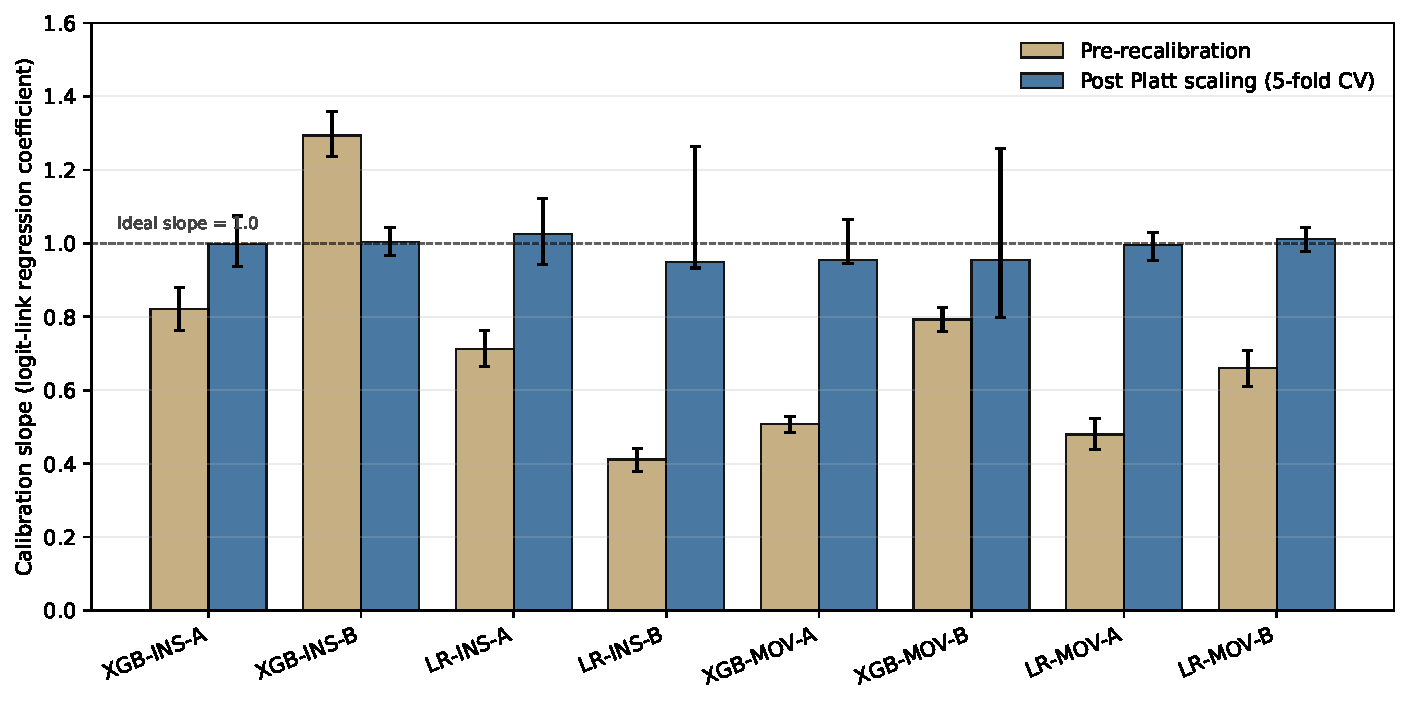
\includegraphics[width=0.95\textwidth]{figures/figure_S5a_calib_slope.pdf}
\caption{Per-model calibration slope before and after Platt scaling. Pre
slopes (tan) span \pnCalibSlopePreRangeFull, with logistic-regression on
the INSPIRE direction (LR-INS-B) at the lowest and XGBoost on the same
direction (XGB-INS-B) at the highest. Post-recalibration slopes (blue) all
include 1.0 within their 95\% bootstrap CIs (\pnCalibSlopePostRangeFull).
Error bars are 2{,}000-resample case-level paired bootstrap CIs.\\[0.5em]{\small\itshape Alt text: Paired-bar chart with eight model panels. For each model, two horizontal bars show calibration slope before Platt-scaling recalibration (tan, with whiskers at the 95\% bootstrap CI) and after recalibration (blue, also with bootstrap CI). The pre-recalibration tan bars span a wide range from 0.41 (LR-INS-B, the worst) to 1.29 (XGB-INS-B, the best), all far from the ideal slope of 1.0. The post-recalibration blue bars cluster tightly between 0.95 and 1.02, with each 95\% CI now including 1.0. The visualization makes immediately visible that Platt scaling restores calibration uniformly across the eight cross-population validation runs.}}
\label{fig:s5-calib-slope}
\end{figure}

\begin{figure}[H]
\centering
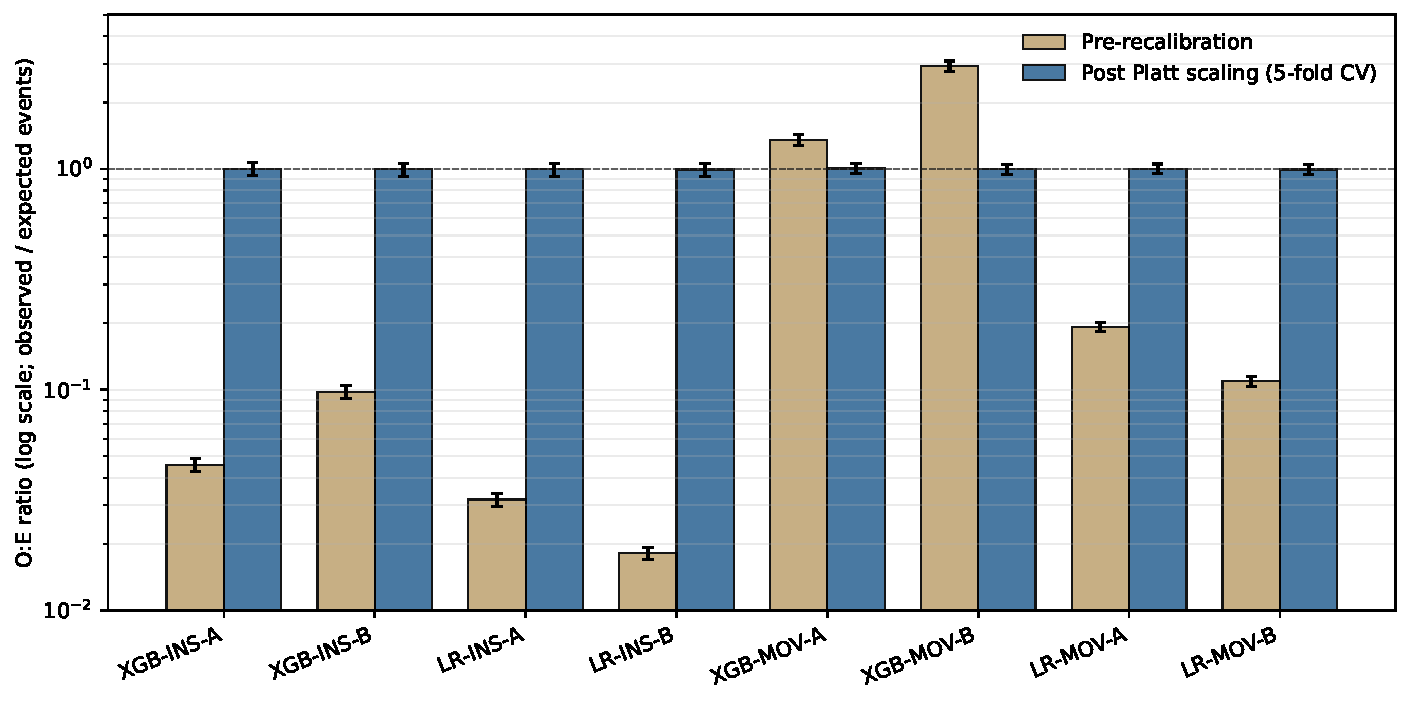
\includegraphics[width=0.95\textwidth]{figures/figure_S5b_oe_ratio.pdf}
\caption{Per-model observed-to-expected (O:E) ratios before and after
Platt scaling, on a logarithmic vertical axis (pre-recal range spans two
orders of magnitude). The direction-asymmetric pre-recal pattern is
visible: INSPIRE-trained on MOVER under-predicts
(\pnOERatioInspireTrainedPreRange); MOVER-trained on INSPIRE
under-predicts (LR variants \pnOERatioMoverTrainedPreRangeLR) or
over-predicts (XGB variants \pnOERatioMoverTrainedPreRangeXGB).
Post-recal: \pnOERatioPostRangeFull. Error bars are 95\% bootstrap CIs.\\[0.5em]{\small\itshape Alt text: Paired-bar chart with eight model panels on a logarithmic vertical axis (pre-recal range spans two orders of magnitude). For each model, two bars show observed-to-expected ratio (O:E) before Platt-scaling recalibration (tan) and after (blue), with 95\% bootstrap CI whiskers. The pre-recalibration tan bars reveal a direction-asymmetric pattern: INSPIRE-trained models on MOVER under-predict mortality (O:E values clustered around 0.02 to 0.10, well below the ideal of 1.0); MOVER-trained models on INSPIRE either under-predict (LR variants, O:E around 0.10 to 0.19) or substantially over-predict (XGB variants, O:E up to 2.92). The post-recalibration blue bars cluster tightly around 1.0 (range 0.99--1.01) for every model. The visualization documents both the direction-asymmetric pre-recal mis-calibration and Platt scaling's uniform corrective effect.}}
\label{fig:s5-oe-ratio}
\end{figure}

\begin{figure}[H]
\centering
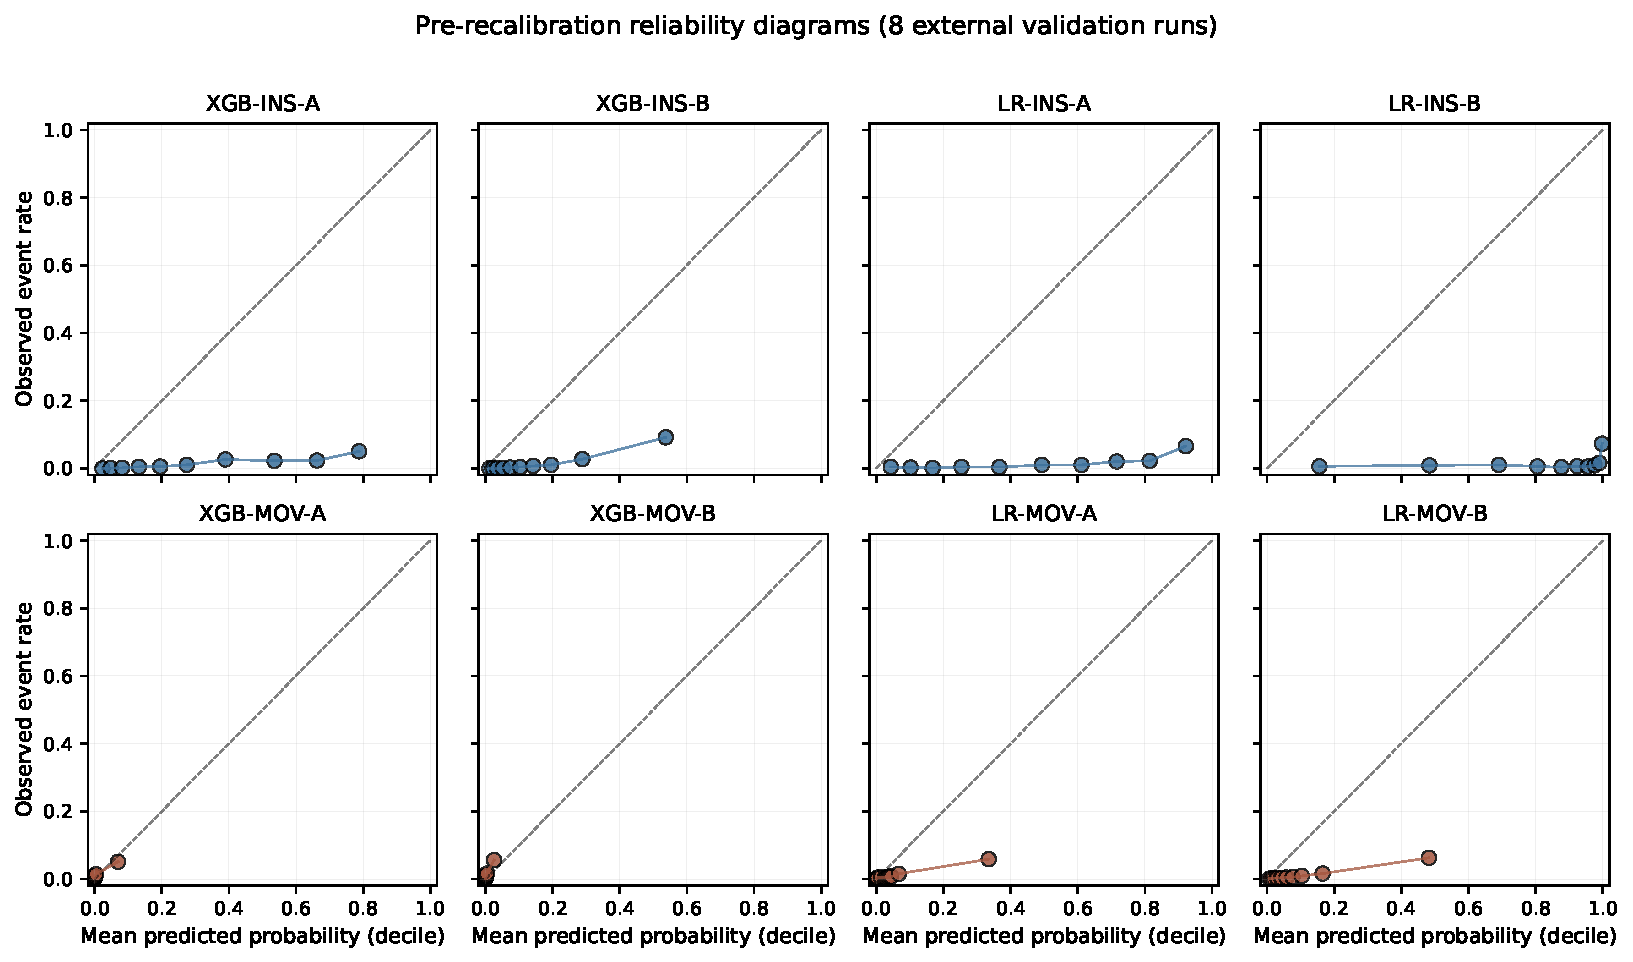
\includegraphics[width=0.96\textwidth]{figures/figure_S5c_calib_curves.pdf}
\caption{Pre-recalibration reliability diagrams for the eight external
validation runs (deciles of predicted probability vs.\ observed event
rate). Marker size scales with bin n. Top row: INSPIRE-trained models
on MOVER (under-prediction visible as observed rates above the diagonal).
Bottom row: MOVER-trained models on INSPIRE (XGB variants over-predict in
the upper deciles; LR variants under-predict). The diagonal is the ideal
calibration line.\\[0.5em]{\small\itshape Alt text: Eight-panel reliability-diagram grid showing pre-Platt-scaling calibration for every external validation run. Within each panel, the horizontal axis is decile of predicted probability and the vertical axis is observed event rate; markers are placed per decile, sized by bin sample count, and the dashed diagonal is the ideal-calibration reference. Top row (INSPIRE-trained models on MOVER): markers consistently lie above the diagonal in the upper deciles, indicating under-prediction of mortality. Bottom row (MOVER-trained models on INSPIRE): the XGB variants show markers above the diagonal in the upper deciles (over-prediction); the LR variants show markers below the diagonal (under-prediction). The grid makes the direction- and algorithm-specific mis-calibration patterns visually inspectable per model.}}
\label{fig:s5-calib-curves}
\end{figure}

\subsection{Inferential robustness}\label{supp:s5-inferential-robustness}

The principal findings reported in main \S2.3--\S2.6 carry their own
case-level paired bootstrap CIs (2{,}000 iterations,
\texttt{seed = 42}; \S\ref{supp:s3-bootstrap}); all bootstrap CIs and
two-sided p-values are reproducible from the cached per-model
predictions documented in main \S3.6 without retraining. The
permutation test on model-level degradation (4-vs-4 split) has minimum
achievable $p = 1/70 \approx 0.014$ (\S\ref{supp:s3-permutation}) and is
floor-bounded irrespective of the underlying effect, which is why
case-level inference is the primary framework. DeLong's asymptotic test
(\S\ref{supp:s3-delong}) is reported as a within-direction sensitivity
check across the four pairwise preop-vs-intraop comparisons; pairwise
significance under Benjamini--Hochberg correction matches the
case-level paired bootstrap conclusions in main \S2.5. Bootstrap-iteration
sensitivity (1{,}000 vs.\ 2{,}000 resamples) and seed sensitivity were
spot-checked during development without producing meaningful
point-estimate or CI shifts; comprehensive sweep tables are not
distributed because the underlying conclusions are determined by
case-count rather than resample-count, and the case counts
(\pnTableOneNInspire\ and \pnTableOneNMover) are large.

\subsection{Data-constrained analyses}\label{supp:s5-data-constrained}

Three analyses we would have run if the data permitted are reported as
constraints rather than results.

\textbf{Race/ethnicity stratification.} The MOVER public release omits
race/ethnicity at the source-data level: the
\texttt{PATIENT\_RACE\_C} and \texttt{PATIENT\_ETHNIC\_C} fields are
absent from the released MOVER EHR data tables (verified directly
against the public release). INSPIRE has no equivalent variable. No race-stratified or ethnicity-stratified discrimination analysis
is therefore possible from the data as released, in either direction, and
no surrogate inference is attempted; the absence is documented as a
data-availability constraint rather than a null result. This is a fairness limitation explicitly recommended-against by
the clinical machine-learning fairness literature~\cite{Chen2020,Pfohl2021}
and is recorded as a primary limitation in main \S4.5.

\textbf{Temporal period matching.} INSPIRE timestamps are
privacy-preserving relative-time offsets without a calendar-date
crosswalk; the 2015--2020 overlap window with MOVER cannot be enforced
(\S\ref{supp:s4-temporal}).

\textbf{Procedure-type matching.} INSPIRE's KCD-10 and MOVER's CPT/EPIC
procedure code taxonomies do not align without a purpose-built crosswalk.
Procedure-type subgroup matching is therefore not attempted.

\subsection{SHAP feature transferability}\label{supp:s5-shap}

Figures~\ref{figS:shap_xgb_ins_b} and \ref{figS:shap_xgb_mov_b} are the
SHAP summary plots for the best XGBoost model in each transfer direction:
XGB-INS-B externally validated on MOVER, and XGB-MOV-B externally
validated on INSPIRE. SHAP-rank ordering is preserved across institutions
with Spearman \pnShapSpearmanRhoXgbInsBFull\ and
\pnShapSpearmanRhoXgbMovBFull\ across all 140 shared features
(main \S2.6); the top-ranked features are ASA, BMI, age, and heart-rate-
derived intraoperative summaries in both directions
(Table~\ref{tab:transferable_features}). The dissociation between
rank-stable feature importance and direction-asymmetric calibration is
the empirical anchor for the ``relational structure transfers, absolute
mappings do not'' interpretation in main \S4.3.

\begin{table}[H]
\centering
\caption{Top-10 transferable features by SHAP rank for the best XGBoost
model in each transfer direction. For each direction, internal rank
(10-fold OOF) and external rank (held-out alternate cohort) are shown;
rank-stability is high in both directions (Spearman $\rho$ across all 140
shared features: \pnShapSpearmanRhoXgbInsBFull\ for XGB-INS-B;
\pnShapSpearmanRhoXgbMovBFull\ for XGB-MOV-B). ASA is rank-1 in both
directions; demographic features (BMI, age) and HR-derived intraoperative
summaries dominate the top 10.}
\label{tab:transferable_features}
\setlength{\tabcolsep}{4pt}
\small
\begin{tabular}{rl@{\hskip 1em}cc@{\hskip 2em}l@{\hskip 1em}cc}
\toprule
& \multicolumn{3}{c}{\textbf{XGB-INS-B (INSPIRE $\to$ MOVER)}}
& \multicolumn{3}{c}{\textbf{XGB-MOV-B (MOVER $\to$ INSPIRE)}} \\
\cmidrule(lr){2-4} \cmidrule(lr){5-7}
\textbf{Rank} & \textbf{Feature} & \textbf{Int.} & \textbf{Ext.} & \textbf{Feature} & \textbf{Int.} & \textbf{Ext.} \\
\midrule
1  & asa            & 1 & 1  & asa                & 1 & 1 \\
2  & bmi            & 2 & 2  & bmi                & 2 & 3 \\
3  & age            & 3 & 4  & age                & 3 & 4 \\
4  & hr\_mean       & 4 & 5  & height\_cm         & 4 & 8 \\
5  & sex            & 5 & 8  & weight\_kg         & 5 & 5 \\
6  & emergency      & 6 & 6  & high\_asa          & 6 & 2 \\
7  & hr\_n          & 7 & 3  & etco2\_std         & 7 & 6 \\
8  & hr\_min        & 8 & 10 & high\_asa\_emergency & 8 & 9 \\
9  & department     & 9 & 12 & hr\_first          & 9 & 12 \\
10 & dbp\_art\_mean & 10 & 13 & hr\_mean           & 10 & 7 \\
\bottomrule
\end{tabular}
\end{table}

\begin{figure}[H]
\centering
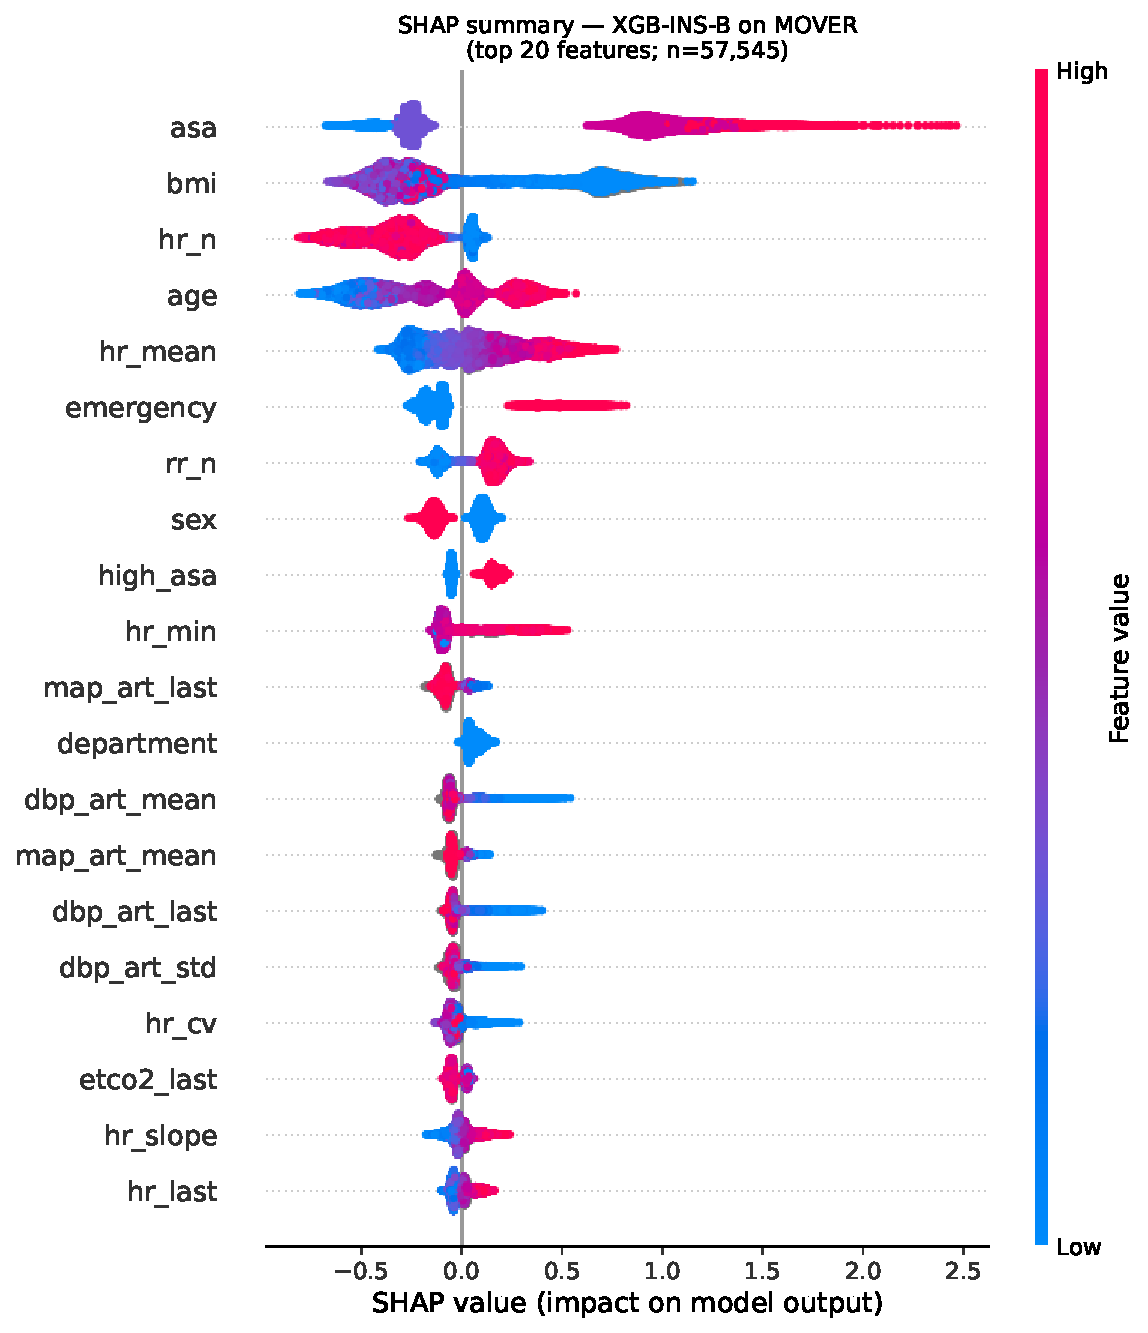
\includegraphics[width=0.95\textwidth]{figures/figure_S5e_shap_xgb_ins_b.pdf}
\caption{SHAP summary plot for XGB-INS-B externally validated on MOVER.
Top-ranked features by mean absolute SHAP value: ASA, BMI, age, and
heart-rate-derived intraoperative summaries. Internal-vs-external
Spearman rank correlation across all 140 shared features:
\pnShapSpearmanRhoXgbInsBFull.\\[0.5em]{\small\itshape Alt text: SHAP summary plot for the best XGBoost intraoperative model trained on INSPIRE and externally validated on MOVER. Vertical axis lists the top-ranked features by mean absolute SHAP value (ASA, BMI, age, then a sequence of heart-rate-derived intraoperative summaries). Horizontal axis is per-case SHAP value (impact on the model's log-odds prediction). Each row shows a swarm of points (one per MOVER patient), colored from blue (low feature value) through red (high feature value), so the plot reveals both feature importance ranking and per-feature directionality of effect. Internal-to-external Spearman rank correlation across all 140 shared features is reported in the figure caption; the rank ordering visible here is preserved relative to the model's INSPIRE training-set ranking.}}
\label{figS:shap_xgb_ins_b}
\end{figure}

\begin{figure}[H]
\centering
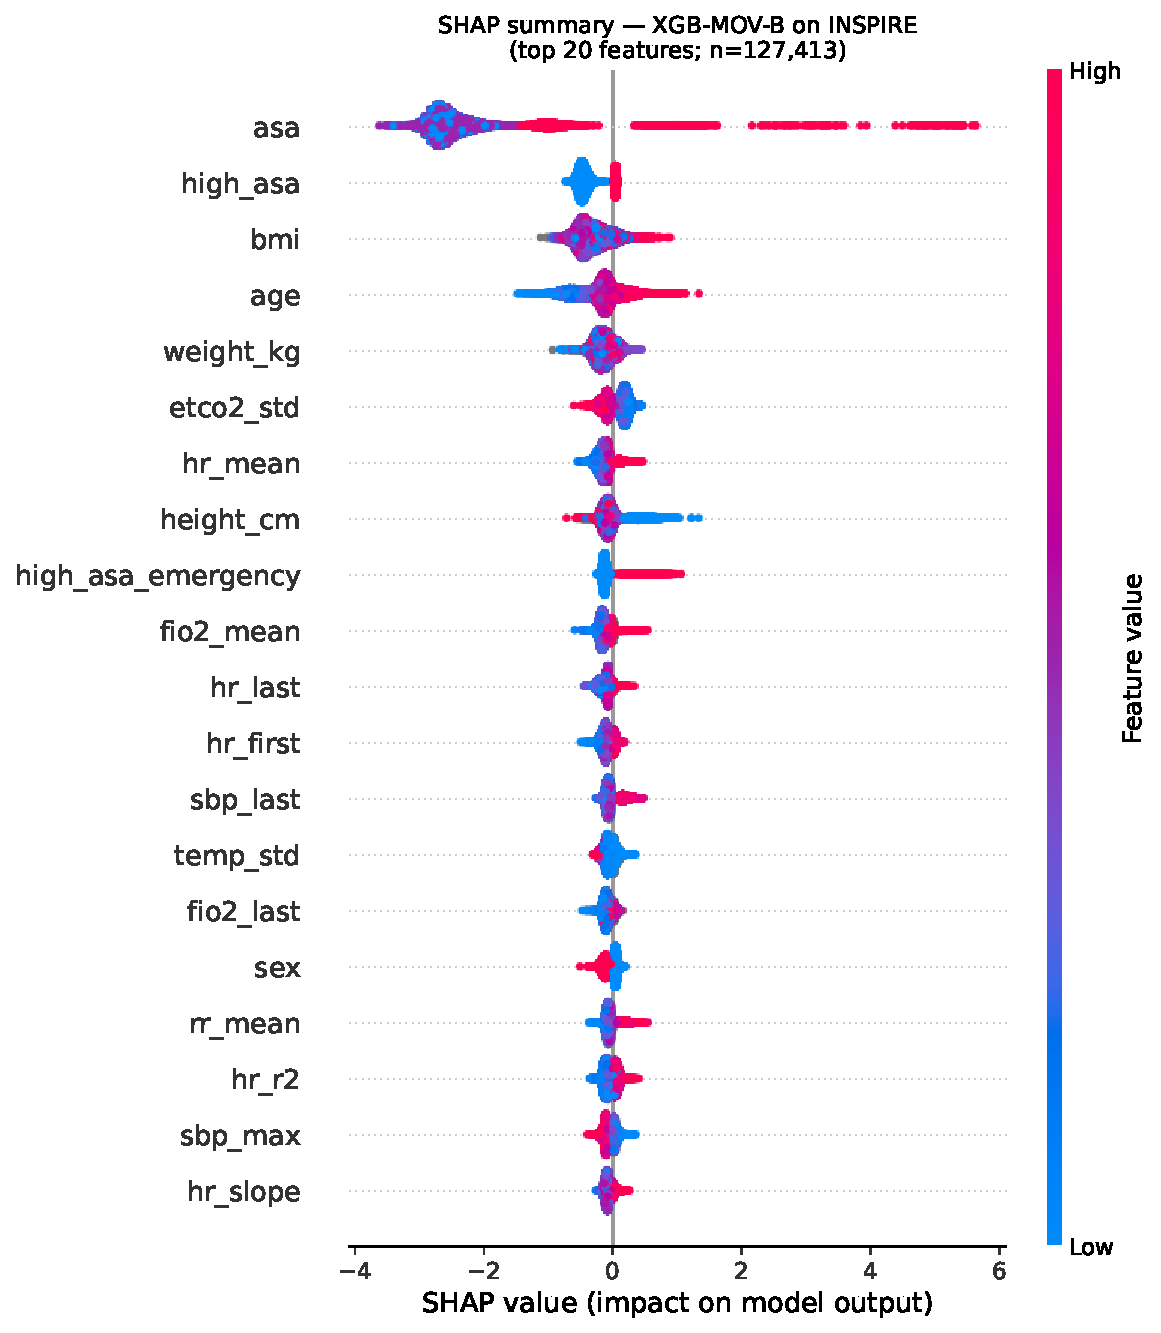
\includegraphics[width=0.95\textwidth]{figures/figure_S5f_shap_xgb_mov_b.pdf}
\caption{SHAP summary plot for XGB-MOV-B externally validated on INSPIRE.
Top-ranked feature ordering matches XGB-INS-B's. Internal-vs-external
Spearman rank correlation across all 140 shared features:
\pnShapSpearmanRhoXgbMovBFull.\\[0.5em]{\small\itshape Alt text: SHAP summary plot for the best XGBoost intraoperative model trained on MOVER and externally validated on INSPIRE --- the reverse direction of the previous figure. Vertical axis lists top-ranked features by mean absolute SHAP value, with the same dominant features (ASA, BMI, age, heart-rate-derived intraoperative summaries) as in the INSPIRE$\to$MOVER direction. Horizontal axis is per-case SHAP value; each row shows a swarm of per-case impact dots colored by feature value (blue = low, red = high). The figure's central finding, when read alongside the previous figure, is that top-feature ordering is preserved across the bidirectional training/test swap.}}
\label{figS:shap_xgb_mov_b}
\end{figure}

\subsection{Decision-curve clinical utility (per-direction detail)}\label{supp:s5-dca}

Figure~\ref{fig:s5-dca-detail} reports per-model decision-curve net
benefit across the \pnDcaThresholdRange\ threshold range; the aggregated
view is in main Figure~\ref{fig:dca}. The per-model breakdown makes the
LR-INS-B utility-loss above 2\% threshold visible (consistent with its
intraoperative-feature underperformance reported in main \S2.5); the other
seven models retain positive net benefit across the full
\pnDcaThresholdRange\ interval.

\begin{figure}[H]
\centering
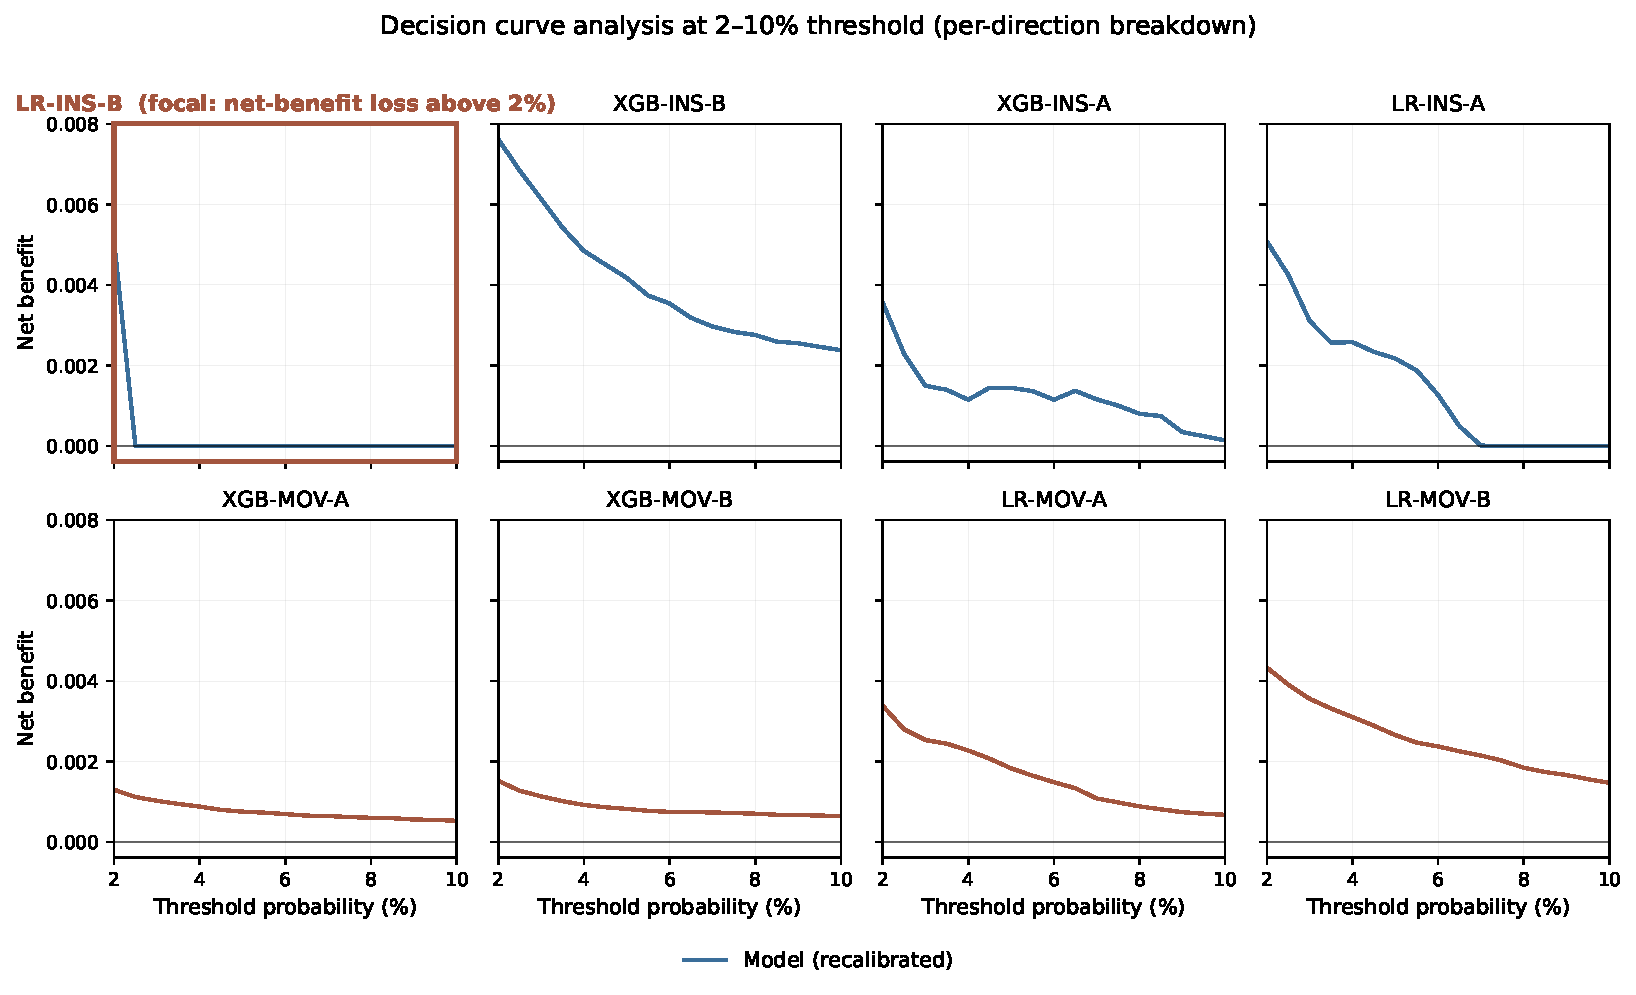
\includegraphics[width=0.96\textwidth]{figures/figure_S5d_dca_per_direction.pdf}
\caption{Per-model decision-curve net benefit at \pnDcaThresholdRange\
threshold (post-Platt-scaling). Top row: INSPIRE-trained models on MOVER;
bottom row: MOVER-trained models on INSPIRE. The LR-INS-B panel
(top-left) is highlighted as the focal deployment-failure case
(net-benefit loss above 2\% threshold).\\[0.5em]{\small\itshape Alt text: Eight-panel decision-curve grid showing post-Platt-scaling per-model net benefit across the clinically relevant 2\%--10\% decision threshold range. Top row: four INSPIRE-trained models on MOVER. Bottom row: four MOVER-trained models on INSPIRE. Within each panel, the model's net-benefit curve is plotted alongside the treat-all reference. Most panels show positive net benefit across the full threshold range. The top-left panel (LR-INS-B) is highlighted as the focal deployment-failure case: net benefit drops below the treat-all reference for thresholds above 2\%, indicating that this specific model, despite recalibration, would harm clinical utility if deployed on MOVER for thresholds in the upper part of the clinically relevant range.}}
\label{fig:s5-dca-detail}
\end{figure}


%% =============================================================================
%% §S6 --- Aggregated statistics for verification
%% =============================================================================
%%
\section{Aggregated statistics for verification}\label{supp:s6-aggregated}

This section provides aggregated, claim-level reference tables that allow
verification of every main-text quantitative claim without redistributed
patient-level data. Each subsection's table is sourced from the canonical
analysis outputs and is consistent with the values reported in main
results; aggregated publication is consistent with both DUAs'
minimum-cell-size requirements.

\subsection{Per-model per-stratum AUCs}\label{supp:s6-stratum-auc}

Table~\ref{tab:s6-stratum-auc} reports per-model overall and within-stratum
external AUCs across two stratification axes (ASA stratum; sex). Cells marked \textsuperscript{a}
flag $n_{\text{events}} < 10$ in that stratum (single-stratum
fallback applies in the paradox-gap calculation; main \S2.3 + Table~\ref{tab:paradox}).

\begin{table}[H]
\centering
\caption{Per-model external AUCs by stratum (overall, ASA 1--2, ASA $\geq 3$,
female, male). Cells marked \textsuperscript{a} flag $n_{\text{events}} < 10$ (MOVER's
ASA 1--2 stratum has 9 deaths).}
\label{tab:s6-stratum-auc}
\setlength{\tabcolsep}{4pt}
\small
\begin{tabular}{lccccc}
\toprule
\textbf{Model} & \textbf{Overall} & \textbf{ASA 1--2} & \textbf{ASA $\geq 3$} & \textbf{Female} & \textbf{Male} \\
\midrule
XGB-INS-A on MOVER  & 0.785 & 0.621\textsuperscript{a} & 0.682 & 0.783 & 0.775 \\
XGB-INS-B on MOVER  & 0.895 & 0.724\textsuperscript{a} & 0.845 & 0.893 & 0.890 \\
LR-INS-A on MOVER   & 0.796 & 0.645\textsuperscript{a} & 0.715 & 0.783 & 0.791 \\
LR-INS-B on MOVER   & 0.741 & 0.858\textsuperscript{a} & 0.687 & 0.737 & 0.733 \\
\midrule
XGB-MOV-A on INSPIRE & 0.756 & 0.597 & 0.584 & 0.748 & 0.755 \\
XGB-MOV-B on INSPIRE & 0.812 & 0.705 & 0.741 & 0.830 & 0.796 \\
LR-MOV-A on INSPIRE  & 0.806 & 0.685 & 0.683 & 0.809 & 0.784 \\
LR-MOV-B on INSPIRE  & 0.839 & 0.746 & 0.771 & 0.848 & 0.819 \\
\bottomrule
\multicolumn{6}{l}{\footnotesize \textsuperscript{a}MOVER ASA 1--2 stratum has $n_{\text{events}} = 9$; AUC reported for completeness, not used in paradox gap.} \\
\end{tabular}
\end{table}

\subsection{Per-model paradox gap summary}\label{supp:s6-paradox-summary}

Table~\ref{tab:paradox_summary} is the paradox gap reference cited from
main \S4.4. It is the same data underlying main Table~\ref{tab:paradox}
(values match exactly); the difference is column structure: this table
reports the gap and its CI in compact form for verification.

\begin{table}[H]
\centering
\caption{Per-model Simpson's paradox gap summary.}
\label{tab:paradox_summary}
\setlength{\tabcolsep}{6pt}
\small
\begin{tabular}{lccccc}
\toprule
\textbf{Model} & \textbf{Trained on} & \textbf{Overall AUC} & \textbf{Within-stratum AUC} & \textbf{Gap (pp)} & \textbf{95\% CI} \\
\midrule
XGB-INS-A & INSPIRE & 0.785 & 0.682 & 10.3 & 9.6--10.9 \\
XGB-INS-B & INSPIRE & 0.895 & 0.845 &  5.0 & 4.4--5.6 \\
LR-INS-A  & INSPIRE & 0.796 & 0.715 &  8.1 & 7.5--8.8 \\
LR-INS-B  & INSPIRE & 0.741 & 0.687 &  5.4 & 4.9--5.8 \\
XGB-MOV-A & MOVER   & 0.756 & 0.590 & 16.5 & 15.1--18.0 \\
XGB-MOV-B & MOVER   & 0.812 & 0.723 &  8.9 & 7.9--10.0 \\
LR-MOV-A  & MOVER   & 0.806 & 0.684 & 12.2 & 10.7--13.6 \\
LR-MOV-B  & MOVER   & 0.839 & 0.759 &  8.0 & 6.8--9.2 \\
\bottomrule
\end{tabular}
\end{table}

\subsection{Per-model calibration metrics}\label{supp:s6-calibration}

The full per-model pre/post Platt calibration metrics (slope, intercept,
O:E, Brier) are in Table~\ref{tab:s5-platt-summary}
(§\ref{supp:s5-per-model}). That table
is the verification-form aggregation backing the \pnCalibSlopePreRangeFull,
\pnCalibSlopePostRangeFull, \pnOERatioPostRangeFull, and
\pnBrierMeanImprovementPct\ summary statistics in main \S2.6.

\subsection{Matched-sensitivity full values}\label{supp:s6-robustness-full}

Table~\ref{tab:robustness_full} expands Supplementary Table~\ref{tab:matched_sensitivity}
(§\ref{supp:s4-results}) with per-direction degradation columns (the matched
mean degradation in INSPIRE-trained vs MOVER-trained groups, separately)
that the asymmetry-only summary in S5 does not show.

\begin{table}[H]
\centering
\caption{Matched direction-asymmetry full values per dimension and framing.
Per-direction degradation columns are mean external AUC degradation across
the four models in each training direction (relative degradation). The
asymmetry column is MOVER-trained mean $-$ INSPIRE-trained mean.}
\label{tab:robustness_full}
\setlength{\tabcolsep}{4pt}
\small
\begin{tabular}{lccccc}
\toprule
\textbf{Dimension} & \textbf{Framing} & \textbf{INS-deg} & \textbf{MOV-deg} & \textbf{Asym (pp)} & \textbf{95\% CI} \\
\midrule
Baseline & unmatched      & 0.054 & 0.139 &  8.53 & 6.91--10.24 \\
ASA      & A1 (INS 90.4/9.6) & $-$0.034 & 0.139 & 17.31 & 12.52--21.60 \\
ASA      & A2 (MOV 36.5/63.5) & 0.054 & 0.170 & 11.56 & 9.69--13.43 \\
ASA      & B (50/50)        & 0.023 & 0.132 & 10.90 & 9.03--12.90 \\
Elixhauser & A1 (MOV 56.7\%)  & 0.054 & 0.150 &  9.65 & 7.98--11.40 \\
Elixhauser & A2 (INS 47.8\%)  & 0.054 & 0.162 & 10.76 & 8.95--12.52 \\
Elixhauser & B (50/50)        & 0.054 & 0.151 &  9.68 & 7.93--11.58 \\
Emergency  & A1 (INS up to 15.6\%) & 0.054 & 0.114 &  6.01 & 4.25--7.93 \\
Emergency  & A2 (MOV down to 7.9\%) & 0.054 & 0.127 &  7.32 & 5.37--9.22 \\
Emergency  & B (midpoint 11.75\%)  & 0.054 & 0.126 &  7.16 & 5.25--9.02 \\
Temporal & ---             & \multicolumn{4}{l}{Infeasible (\S\ref{supp:s4-temporal})} \\
\bottomrule
\end{tabular}
\end{table}

\subsection{Sex-stratified AUCs}\label{supp:s6-sex-stratified}

Per-model sex-stratified external AUCs with 95\% bootstrap CIs and
$|F-M|$ differential. The 5-pp threshold pre-specified for fairness flags
(main \S2.7) was not exceeded by any model.

\begin{table}[H]
\centering
\caption{Per-model sex-stratified external AUCs. $|F-M|$ pp is the absolute
female-male AUC differential in percentage points.}
\label{tab:sensitivities}
\setlength{\tabcolsep}{4pt}
\small
\begin{tabular}{lccccc}
\toprule
\textbf{Model} & \shortstack{\textbf{Female AUC}\\\textbf{(95\% CI)}} & \shortstack{\textbf{$n_F$}\\\textbf{events}} & \shortstack{\textbf{Male AUC}\\\textbf{(95\% CI)}} & \shortstack{\textbf{$n_M$}\\\textbf{events}} & \shortstack{\textbf{$|F\!-\!M|$}\\\textbf{pp}} \\
\midrule
XGB-INS-A on MOVER  & \shortstack{0.783\\(0.761--0.803)} & 264 & \shortstack{0.775\\(0.757--0.792)} & 559 & 0.8 \\
XGB-INS-B on MOVER  & \shortstack{0.893\\(0.875--0.908)} & 264 & \shortstack{0.890\\(0.878--0.901)} & 559 & 0.3 \\
LR-INS-A on MOVER   & \shortstack{0.783\\(0.754--0.812)} & 264 & \shortstack{0.791\\(0.772--0.810)} & 559 & 0.7 \\
LR-INS-B on MOVER   & \shortstack{0.737\\(0.697--0.776)} & 264 & \shortstack{0.733\\(0.707--0.757)} & 559 & 0.4 \\
XGB-MOV-A on INSPIRE & \shortstack{0.748\\(0.723--0.771)} & 520 & \shortstack{0.755\\(0.736--0.773)} & 867 & 0.7 \\
XGB-MOV-B on INSPIRE & \shortstack{0.830\\(0.811--0.849)} & 520 & \shortstack{0.796\\(0.780--0.811)} & 867 & 3.4 \\
LR-MOV-A on INSPIRE  & \shortstack{0.809\\(0.788--0.830)} & 520 & \shortstack{0.784\\(0.767--0.800)} & 867 & 2.6 \\
LR-MOV-B on INSPIRE  & \shortstack{0.848\\(0.828--0.865)} & 520 & \shortstack{0.819\\(0.804--0.833)} & 867 & 2.8 \\
\bottomrule
\end{tabular}
\end{table}

\subsection{Bootstrap iteration-count sensitivity}\label{supp:s6-bootstrap-sensitivity}

The headline direction-asymmetry case-level paired bootstrap was re-run at
$B = 500$ and $B = 1{,}000$ in addition to the canonical $B = 2{,}000$
(Table~\ref{tab:s6-iteration-sweep}). Point estimates and CI bounds are
stable across resample counts; CI width narrows as $B$ increases but the
inferential conclusion (asymmetry $> 0$ at the Monte Carlo floor
$p = 0.001$, \S\ref{supp:s3-mc-floor}) does not depend on the resample
count at the case-level $n$ used here.

\begin{table}[H]
\centering
\caption{Bootstrap iteration-count sensitivity for the headline direction-
asymmetry claim, computed at $B = 500$, $B = 1{,}000$, and $B = 2{,}000$ from
the cached per-model predictions using the paired-bootstrap engine
described in \S\ref{supp:s3-bootstrap}.}
\label{tab:s6-iteration-sweep}
\setlength{\tabcolsep}{6pt}
\small
\begin{tabular}{ccccc}
\toprule
\textbf{$B$} & \textbf{Point estimate (pp)} & \textbf{95\% CI lower (pp)} & \textbf{95\% CI upper (pp)} & \textbf{CI width (pp)} \\
\midrule
500    & 8.52 & 6.84 & 10.11 & 3.27 \\
1{,}000 & 8.53 & 6.84 & 10.19 & 3.35 \\
2{,}000 & 8.53 & 6.85 & 10.25 & 3.40 \\
\bottomrule
\end{tabular}
\end{table}


%% =============================================================================
%% §S7 --- Healthcare-system mechanism evidence
%% =============================================================================
\section{Healthcare-system mechanism evidence}\label{supp:s7-mechanism-evidence}

This section provides the supporting evidence for the healthcare-system
mechanism interpretation introduced in main \S4.3. The data anchor (a
\pnMortalitySplitDifferencePp-pp split-difference between INSPIRE's
spectrum-distributed and MOVER's high-acuity-concentrated mortality
patterns at matched ASA stratum) is established in main \S4.3; here we
report the 2$\times$2 stratified mortality table that backs it
(\S\ref{supp:s7-stratified-mortality}) and expand the cross-institutional
end-of-life-practice literature that grounds the
healthcare-system-specific feature--outcome-mapping interpretation
(\S\ref{supp:s7-eol-practice}). Cross-references to the matched-case-mix
analysis are in \S\ref{supp:s7-residual}.

\subsection{Stratified mortality distribution}\label{supp:s7-stratified-mortality}

The full distribution of in-hospital deaths by ASA stratum across the two
cohorts is in Table~\ref{tab:s7-stratified-mortality}. INSPIRE deaths
spread across the acuity spectrum (\pnTableOneDeathsAsaOneTwoPctInspire\
in ASA 1--2 vs \pnTableOneDeathsAsaThreePlusPctInspire\ in ASA $\geq 3$),
whereas MOVER deaths concentrate almost entirely in high-acuity patients
(1.1\% in ASA 1--2 vs \pnTableOneDeathsAsaThreePlusPctMover\ in ASA
$\geq 3$). The corresponding within-stratum mortality rates also diverge
markedly: INSPIRE ASA 1--2 rate 0.57\% (654 deaths over
\pnTableOneAsaOneTwoInspire\ surgeries) vs MOVER ASA 1--2 rate 0.04\% (9
deaths over \pnTableOneAsaOneTwoMover); INSPIRE ASA $\geq 3$ rate 5.97\%
(733 deaths over \pnTableOneAsaThreePlusInspire) vs MOVER ASA $\geq 3$
rate 2.23\% (814 deaths over \pnTableOneAsaThreePlusMover). The
mortality-share split between the two strata is therefore not a small
perturbation; it is structural.

\begin{table}[H]
\centering
\caption{Stratified in-hospital mortality distribution by cohort and ASA
stratum. Cells report deaths $n$, share-of-deaths within cohort, and
within-stratum mortality rate.}
\label{tab:s7-stratified-mortality}
\setlength{\tabcolsep}{6pt}
\begin{tabular}{lll}
\toprule
\textbf{Cohort} & \textbf{ASA 1--2 deaths} & \textbf{ASA $\geq 3$ deaths} \\
\midrule
INSPIRE & \pnTableOneDeathsAsaOneTwoInspire & \pnTableOneDeathsAsaThreePlusInspire \\
MOVER  & \pnTableOneDeathsAsaOneTwoMover  & \pnTableOneDeathsAsaThreePlusMover \\
\bomark
\end{tabular}
\end{table}

\subsection{Cross-institutional end-of-life practice patterns}\label{supp:s7-eol-practice}

End-of-life decision-making practices in intensive care units differ
systematically between East Asian and Western settings, and these
differences may shape the joint distribution of physiological
trajectories and observed in-hospital mortality outcomes. Phua and
colleagues~\cite{Phua2015} surveyed end-of-life practices across 16 Asian
countries and territories (including South Korea), reporting that the
proportion of deaths preceded by withholding or withdrawing
life-sustaining treatments was substantially lower than that documented
in contemporaneous Western studies, and that withdrawing (as distinct
from withholding) was particularly uncommon in many Asian sites. Within
South Korea specifically, Park and colleagues~\cite{Park2018} described
sharp temporal shifts in withdrawing/withholding practices coincident
with the introduction of the Act on Hospice and Palliative Care
(implemented 2018), and documented that, even after the legal change,
attending-physician discretion and family-centric decision frameworks
remained associated with substantial inter-institutional variability in
EOL care patterns. The \pnMortalitySplitDifferencePp-pp split-difference
between INSPIRE's spectrum-distributed and MOVER's high-acuity-concentrated
mortality patterns (main \S4.3; \S\ref{supp:s7-stratified-mortality}) is
consistent with this class of practice variability, though our data alone
cannot identify any specific mechanism.

\subsection{Implication for the residual asymmetry}\label{supp:s7-residual}

The matched-case-mix sensitivity analysis (\S\ref{supp:s4-matched})
established that approximately 70\% of the unmatched
direction-asymmetry baseline survives matching on three testable
case-mix dimensions (ASA, Elixhauser comorbidity, emergency-case
proportion). This residual asymmetry is consistent with
healthcare-system-specific feature--outcome relationships that case-mix
matching does not equalize --- both because some sources of asymmetry
(temporal period; \S\ref{supp:s4-temporal}) cannot be matched, and
because some sources operate within strata in ways inter-rater-variable
ASA classification~\cite{Sankar2014} does not capture. The cross-
institutional EOL-practice patterns reviewed in
\S\ref{supp:s7-eol-practice} are one plausible mechanism class among
several; our cohort data cannot directly distinguish among candidate
mechanisms. The interpretation in main
\S4.3 is therefore framed as ``consistent with'' rather than
``established by'' the available data.


%% =============================================================================
%% §S8 --- TRIPOD+AI reporting checklist
%% =============================================================================
\section{TRIPOD+AI reporting checklist}\label{supp:s8-tripod-checklist}

This section maps the manuscript against the TRIPOD+AI reporting
checklist (Collins et al.~2024)~\cite{Collins2024}. Items 1--27 cover
the full development--evaluation lifecycle; this study is an evaluation
study (cross-cohort external validation of pre-trained models from
INSPIRE / MOVER public data releases). For items that primarily concern
model development, the relevant content is reported in Methods §3.2 +
Supplementary §S2 (which document the development pipeline our analyses
re-use).

\renewcommand{\arraystretch}{1.05}
\begin{longtable}{p{0.06\textwidth}p{0.32\textwidth}p{0.55\textwidth}}
\caption{TRIPOD+AI reporting checklist (Collins et al.\ 2024) mapped to
manuscript sections. ``Main \S X'' refers to canonical Methods/Results/
Discussion sections; ``Supp \S Y'' refers to numbered subsections in this
supplementary file.}
\label{tab:s8-tripod-checklist}\\
\toprule
\textbf{Item} & \textbf{Topic} & \textbf{Manuscript reference} \\
\midrule
\endfirsthead

\multicolumn{3}{l}{\small\textit{(continued from previous page)}} \\
\toprule
\textbf{Item} & \textbf{Topic} & \textbf{Manuscript reference} \\
\midrule
\endhead

\midrule
\multicolumn{3}{r}{\small\textit{(continued on next page)}} \\
\endfoot

\bottomrule
\endlastfoot

\multicolumn{3}{l}{\textbf{Title and Abstract}} \\
1   & Identify the study as developing/evaluating a prediction model & Title; Abstract Objective \\
2   & Structured abstract (Objective, Methods, Results, Conclusion) & Abstract \\
\midrule
\multicolumn{3}{l}{\textbf{Introduction}} \\
3a  & Healthcare context and rationale & Main §1 (Background) \\
3b  & Target population, intended purpose, intended users & Main §1; §4.4 (Clinical implications) \\
3c  & Known health inequalities between sociodemographic groups & Main §4.5 (Limitations); Supp §S5.3 (Race/ethnicity unavailability) \\
4   & Study objectives (development vs evaluation) & Main §1 closing paragraph; this is an evaluation study \\
\midrule
\multicolumn{3}{l}{\textbf{Methods}} \\
5a  & Data sources, separately for dev / eval, with representativeness & Main §3.1; Supp §S1.1, §S1.2 \\
5b  & Dates of data collection (accrual + follow-up) & Main §3.1 (INSPIRE 2011--2020; MOVER 2015--2022) \\
6a  & Study setting, number/location of centres & Main §3.1 (single-centre each cohort) \\
6b  & Eligibility criteria for participants & Main §3.1; Supp §S1.1, §S1.2; main Figure~\ref{fig:cohort} \\
6c  & Treatments received and how handled & N/A (cross-cohort EHR-based study; no treatment intervention) \\
7   & Data pre-processing and quality checks across groups & Main §3.1; Supp §S2.1 (feature inventory + completeness rates) \\
8a  & Outcome definition, time horizon, assessment method & Main §3.1 (in-hospital mortality) \\
8b  & Outcome assessor qualifications (if subjective) & N/A (administrative outcome ascertainment) \\
8c  & Outcome assessment blinding & N/A \\
9a  & Predictor pre-selection before model building & Main §3.2; Supp §S2.1 (8 preop, 132 intraop) \\
9b  & Predictor definitions, measurement timing, blinding & Main §3.2 (60-min post-induction window); Supp §S2.1 \\
9c  & Predictor assessor qualifications & N/A (sensor-derived data) \\
10  & Sample size determination and justification & Main §3.2 (EPV ratios stated inline) \\
11  & Missing data handling & Main §3.2; Supp §S2.1 (intraop coverage 99.9\% INSPIRE / 92.1\% MOVER); §S2.2 (mean imputation for LR) \\
12a & Data partitioning for analyses & Main §3.2 (10×5 nested CV); Supp §S2.2 \\
12b & Predictor handling (transformation, scaling) & Supp §S2.2 (LR standardisation; XGBoost native handling) \\
12c & Model type, building steps, hyperparameter tuning & Main §3.2; Supp §S2.2 (full search space + median tuned) \\
12d & Cluster heterogeneity handling & N/A (no clustered structure beyond cohort) \\
12e & Performance evaluation measures & Main §3.3, §3.5; Supp §S3, §S5 \\
12f & Model updating during evaluation & N/A (frozen models; only Platt recalibration; Supp §S3.5) \\
12g & Prediction calculation for evaluation & Main §3.5; Supp §S3.5 \\
13  & Class imbalance methods + recalibration & Main §3.2 + §3.7; Supp §S2.3, §S3.5 \\
14  & Model fairness approaches & Main §2.7 (sex stratification); Supp §S5.3, §S6.5 \\
15  & Model output type and threshold rationale & Main §3.5; main §2.7 (DCA at 2--10\%) \\
16  & Differences between development and evaluation data & Main §2.1, §2.4; Table~\ref{tab:populations} \\
17  & Ethics committee and consent & Main §3.1 (public credentialed-access datasets; separate IRB approvals at source institutions) \\
\midrule
\multicolumn{3}{l}{\textbf{Open Science}} \\
18a & Funding source and funder role & Main Acknowledgments / Funding [forthcoming at submission] \\
18b & Conflicts of interest & Main Disclosures [forthcoming at submission] \\
18c & Study protocol availability & Main §3.6 (no pre-registered protocol; canonical analysis pipeline + scripts under MIT) \\
18d & Study registration & Not registered (post-hoc external-validation study of public datasets) \\
18e & Data availability & Main §3.6 (DUA-Posture-2 commitment; Supp §S6 aggregated tables) \\
18f & Analytical code availability & Main §3.6; Zenodo deposit (DOI assigned at submission) \\
\midrule
\multicolumn{3}{l}{\textbf{Patient and Public Involvement}} \\
19  & PPI in design / conduct / reporting & N/A (secondary use of pre-existing public datasets) \\
\midrule
\multicolumn{3}{l}{\textbf{Results}} \\
20a & Participant flow, outcome numbers, follow-up & Main §2.1; main Figure~\ref{fig:cohort}; Table~\ref{tab:populations} \\
20b & Characteristics overall and by data source & Table~\ref{tab:populations} \\
20c & Comparison of development vs evaluation data distribution & Main §2.1; Supp §S6.1 \\
21  & Participant and event numbers in each analysis & Tables~\ref{tab:paradox} + \ref{tab:asymmetry} + \ref{tab:s6-stratum-auc} \\
22  & Full prediction model details (enabling third-party use) & Main §3.6; Supp §S2 + §S6; Zenodo \\
23a & Performance with CIs, including key subgroups & Main §2.3--§2.7; Supp §S5, §S6.1, §S6.5 \\
23b & Heterogeneity across clusters & Main §2.4 (matched-case-mix); Supp §S4 \\
24  & Model updating results (if any) & Main §2.6 (Platt recalibration); Supp §S5.1, §S6.3, Table~\ref{tab:s5-platt-summary} \\
\midrule
\multicolumn{3}{l}{\textbf{Discussion}} \\
25  & Overall interpretation, fairness, prior studies & Main §4.1, §4.2, §4.3 \\
26  & Limitations, bias, uncertainty, generalisability & Main §4.5; Supp §S5.3 \\
27a & Handling of poor-quality input data at deployment & Main §4.4 (recalibration on representative deployment sample) \\
27b & User interaction with input data & Main §4.4 (TRIPOD+AI-aligned reporting commitments) \\
27c & Next steps for research & Main §4.4, §4.5 \\
\end{longtable}


%% =============================================================================
%% =============================================================================
\bibliographystyle{plainnat}
\bibliography{references}

\end{document}
